\documentclass[12pt]{article}

\usepackage[margin=1in]{geometry}
\usepackage[utf8]{inputenc}
\usepackage[colorlinks]{hyperref}
\usepackage{multirow}
\usepackage{booktabs}
\usepackage{amsmath}
\usepackage{verbatim}
\usepackage{setspace, caption, subcaption, footnote}
\onehalfspacing

\usepackage{footmisc}
%\renewcommand{\footnotesize}{\fontsize{12pt}{12pt}\selectfont\doublespacing}
%\setlength{\footnotesep}{\baselineskip}

\usepackage{graphicx}
\usepackage{tabularx}
\usepackage{indentfirst}
%\usepackage{subfigure}
%\usepackage{apacite}
\usepackage{natbib}
\setcitestyle{aysep={}}					%remove comma between author and year when using citep{}.
\usepackage{color}
\usepackage{longtable}
\usepackage[titletoc,title]{appendix}
\usepackage{lscape}
\usepackage{pdflscape}
\usepackage{subcaption}
\usepackage{caption}
\newcommand{\annote}[1]{\parbox{\textwidth}{\renewcommand{\baselinestretch}{1.0}\vspace{12pt} \footnotesize Notes: #1}}
%\newcommand{\annote}[1]{\parbox{\textwidth}{\renewcommand{\baselinestretch}{2.0}\vspace{12pt} \normalsize Notes: #1}}
\renewcommand{\vec}[1]{\mathbf{#1}}
\usepackage[usenames,dvipsnames,svgnames,table]{xcolor}
\usepackage{hyperref}
\usepackage{libertine}

\hypersetup{
     colorlinks   = true,
     urlcolor	  = black,
     citecolor    = black,
     linkcolor 	  = black
}

\title{\textbf{Monetary Policy and the Wage Inflation-Unemployment Tradeoff}}
\author{Ricardo Duque Gabriel\footnote{\scriptsize Email: \href{mailto:ricardofilipeduquegabriel@gmail.com}{ricardofilipeduquegabriel@gmail.com}. I am grateful to the editors Ambrogio Cesa-Bianchi and Evi Pappa and to two anonymous referees for many valuable comments. I am indebted to Ana Sofia Pessoa, Andreas Westermark, Christian Bayer, David Vestin, Donghai Zhang, Farzad Saidi, Felipe Valencia, Felix Ward, Francisco Amaral, Jean-Pierre Tabin, Joachim Jungherr, João Ritto, Julien Champagne, Kai Arvai, Leonardo Melosi, Lorenzo Ranaldi, Mario Izquierdo, Mathias Klein, Maximilian Jager, Maximilian Weiss, Moritz Schularick, Nuno Palma, Richard Hornbeck, and Roberto Billi for their helpful comments and discussions. I likewise thank seminar participants at the University of Bonn as well as participants at the IZA Workshop: Labor Markets and the Phillips Curve: What Has Changed in the Past 60 Years?, Royal Economic Society 2021 Annual Conference, VI Banco de España Seminar in Economic History, $25^{th}$ Spring Meeting of Young Economists, $4^{th}$ Bonn-Mannheim PhD Workshop, $24^{th}$ Central Bank Macroeconomic Modeling Workshop in Chile, $40^a$ Conferência da Associação Portuguesa de História Económica e Social (best paper award), and $52^{nd}$ Annual Conference of the Money, Macro and Finance Society. I would also like to thank the Sveriges Riksbank and the NBER for hosting me while conducting part of the research that led to this paper. This version supersedes the previously circulating version "Historical Wage Phillips Curves". Finally, I acknowledge financial support from the FCT - Fundação para a Ciência e Tecnologia under the project Ref. SFRH/BD/144581/2019, from the Peter G. Peterson Foundation, and from the Deutsche Forschungsgemeinschaft (DFG, German Research Foundation) under Germany's Excellence Strategy - EXC 2126/1 - 390838866 and also under the RTG 2281 - The Macroeconomics of Inequality.}\\ University of Bonn and NBER}

\date{April 2023}

%\doublespacing
\begin{document}

\begin{titlepage}

\thispagestyle{empty}
\maketitle

\begin{abstract}
\normalsize Using newly assembled data for 18 advanced economies between 1870 and 2019, I study how monetary policy affects wage inflation and unemployment and document two key findings regarding their tradeoff. First, the wage Phillips curve displays a time-varying slope. Second, the tradeoff becomes weaker in low price inflation environments due to a more pronounced unemployment response to monetary policy. These findings lend support to the idea that monetary policy has state-dependent effects with the central banks' ability in exploring the tradeoff being impaired by a low price inflation environment.

%Using newly assembled data for 17 advanced economies between 1870 and 2016 and local projection methods to study how monetary policy affects wage inflation and unemployment, I document two key findings regarding the inflation-unemployment tradeoff. First, the wage Phillips curve displays a time-varying slope. Second, the tradeoff becomes weaker in low price inflation environments due to a muted wage inflation response to monetary policy. These findings lend support to the idea that monetary policy has state-dependent effects with the central banks' ability in exploring the tradeoff being impaired by a low price inflation environment.

%The recent weakening of the inflation-unemployment tradeoff has instigated a debate on whether the New Keynesian framework has outlived its usefulness. Understanding the source of that structural change is crucial for proper monetary policy conduction.  I estimate the inflation-unemployment tradeoff using newly assembled data on wages and unemployment rates for 17 advanced economies since 1870. I show that the wage Phillips curve has always been ``alive and well" despite displaying a time-varying slope. Using the Phillips multiplier framework, I show that the tradeoff becomes weaker in low price inflation environments due to a muted wage inflation response to monetary policy.
\end{abstract}

\vspace{1em}

\textbf{JEL classification:} E24, E31, E52, N10. 

\vspace{1em}

\textbf{Keywords:} Phillips curve, Phillips multiplier, wage inflation, unemployment, monetary policy, economic history 

\end{titlepage}

\clearpage

\begin{quote}
\textit{The relationship between the slack in the economy or unemployment and inflation was a strong one 50 years ago ... and has gone away. (...) At the end of the day, there has to be a connection because low unemployment will drive wages up.} \cite{Powell2019}
\end{quote}


\section{Introduction}
The wage inflation-unemployment tradeoff claims that changes in monetary policy push wage inflation and unemployment in opposite directions \citep{Mankiw2001}. Such relation is traditionally thought of in the form of a Phillips curve and is at the core of monetary policy \citep{Barnichon2019, Eser2020}. Over the last decade, many have questioned the importance of the Phillips curve, arguing that it had flattened out of favor. A flatter Phillips curve suggests that economic activity has a smaller effect on inflation. Under this scenario, central bankers' ability to steer inflation with policy-induced changes becomes weaker. Nevertheless, is this weaker wage inflation-unemployment tradeoff unique to the last two decades? Does the strength of the tradeoff vary over time and differ across states of the economy?


%Most economists recognize its existence, and central bankers rely on it to ``transform" unemployment into inflation by making use of their policy interest rates 

In this study, I revisit the historical relationship between wage inflation and unemployment, which is the focus of Phillips' (\citeyear{Phillips1958}) original work, to answer these two questions. My analysis proceeds in four steps. First, I assemble annual historical data on nominal wages and unemployment rates since 1870 for 18 advanced economies. Second, I uncover considerable variation in the wage Phillips curve slope over time and find that its recent flattening is not a unique feature of the last 150 years. Third, I show that monetary interventions have large and significant effects on wage inflation and unemployment rates. To do so, I take an instrumental variable approach based on the trilemma of international finance, taking advantage of the fact that economies with fixed exchange rates and under perfect capital mobility are unable to implement independent monetary policies and thus, need to mimic the interest rate changes in the pegged country. Finally, I show that the price inflation environment possibly shapes the wage inflation-unemployment tradeoff. Data suggest that the tradeoff is weaker in times of low price inflation, which is consistent with a standard New Keynesian model's predictions \citep{Benati2007}.

I start by reporting time-varying estimates of a micro-founded panel wage Phillips curve, in the spirit of \cite{Gali2011}. I provide evidence that the wage Phillips curve has always been ``alive and well" and that the recent weakening of the wage inflation-unemployment tradeoff is not a unique feature of the last 20 years and can be observed during the Gold Standard periods. Therefore, it is essential to use historical data to better understand what shapes the relationship between these two macroeconomic variables. Furthermore, I find that there is a correlation between periods characterized by a low price inflation environment and a flatter slope.

These results carry on in a setting without the straitjacket of any assumed functional relation between wage inflation and unemployment. To be precise, I estimate a Phillips multiplier in the spirit of \cite{Barnichon2019}, which is related to the impulse response-based statistic presented in \cite{Gali2019}. The main idea is to trace the evolution over time of the dynamic wage inflation-unemployment multiplier by comparing their impulse response functions to a monetary policy shock. While on impact the multiplier is undetermined, at longer horizons the statistic becomes negative and statistically significant. Such a large negative tradeoff implies that a transitory policy-induced change in unemployment has a persistent effect on wage inflation and therefore, that central banks have sufficient ability to steer inflation with conventional monetary policy tools.

Finally, I test the hypotheses that the wage inflation-unemployment tradeoff is different across sub-samples using a state-dependent local projection instrumental variable approach. Results support the hypothesis that, at longer horizons, the tradeoff is smaller during periods of low price inflation. Thus, reinforcing the idea that policymakers' ability to explore such a tradeoff is impaired in a low price inflation environment.

By revisiting the historical relationship between wage inflation and unemployment, this paper aims at contributing to three strands of literature. First, this study adds to the classical literature of the Phillips curve \citep{Phillips1958}. Using long-run data for a panel of 18 countries, I expand the findings of a Phillips curve which is ``alive and well" documented not only for the United States \citep{Coibion2015, Blanchard2016, Hoynck2020, DelNegro2020, Ascari2021, Hazell2021, Bergholt2023} but also in Europe \citep{Levy2019, Onorante2019, Bonam2021} and even worldwide \citep{Coibion2019}.\footnote{A good summary of the literature since the inception of the Phillips curve can be found in \cite{Gordon2011}, while more recent discussions can be found in \cite{Mavroeidis2014} and \cite{Coibion2018}.} 

In the current empirical literature, there is a large amount of sampling uncertainty with different researchers using different data vintages to compute Phillips curves \citep{Mavroeidis2014}. This work introduces two newly assembled historical data series on unemployment rates and wages for a set of 18 countries and an identification strategy based on an instrumental variable approach in the hope of taking one step further to an empirical consensus. The use of such a long-run panel is important because it allows for uncovering the time-varying nature of the tradeoff and that the inflation environment is a historical driver of the wage inflation-unemployment tradeoff. Moreover, it also allows exploring more variation in wage inflation, thereby reducing the results' sensitivity to the data vintage that arises when using recent data. Such an approach keeps up with the recent trend of using long-run and cross-country perspectives to inform central debates in monetary and financial policy as in \cite{Reinhart2009} and \cite{Schularick2012} while bringing a historical perspective to the debate on the wage inflation-unemployment tradeoff.

This work also contributes to the literature about the effects of monetary policy using long-run panel data \citep{Jorda2019, Alpanda2019}. By using the trilemma instrumental variable (IV) to identify the effect of monetary policy, I build not only on the seminal work of \cite{DiGiovanni2009} but also on recent studies by \cite{Jorda2019} and \cite{Schularick2020}. Moreover, this paper applies the Phillips multiplier statistic which was first presented in the study of \cite{Barnichon2019} who estimated it for the US and the UK. This paper's novelty lies in applying the state-of-art methodology to a historical setting with long-run data series that allows testing the response of wage inflation and unemployment rates to a monetary policy surprise, and whether these responses are state-dependent.

Finally, this paper's empirical findings resonate with recent theoretical developments that link the wage inflation-unemployment tradeoff to the level of price inflation. According to a standard New Keynesian model, an increase (decrease) in trend inflation should cause an increase (decrease) in the frequency of price adjustment, leading to a decrease (increase) in the steepness of the wage Phillips curve \citep{Benati2007}. This rationale that low price inflation weakens the wage inflation-unemployment tradeoff is consistent with two other strands of the literature, namely the state-dependent pricing \citep{Alvarez2019, Costain2022} and the nominal price rigidities literatures \citep{Tobin1972, Benigno2011, Daly2014}. Moreover, this rationale is also consistent with the recent view that post-Covid, as the frequency of price changes has increased, we are moving from a flatter to a steeper Phillips curve \citep{Waller2023}.

Since \cite{Ball1988}, the empirical literature has not paid enough attention to this low price inflation mechanism. Some notable exceptions are \cite{Benati2007}, who documented a positive correlation between the time-varying average gain of real activity and inflation; \cite{Vavra2014B}, who rejected a New Keynesian Phillips curve with constant inflation output tradeoff in favor of a slope that increases with microeconomic volatility; \cite{Gertler2018}, who found a weak money-inflation link in regimes characterized by low inflation; and \cite{Ascari2021, Ascari2022} who provide evidence supporting non-linear effects in the response of the price level depending on the trend inflation regime. I complement these findings by showing a negative and strong historical correlation between a time-varying Phillips curve and price inflation, and also by estimating a weaker wage inflation-unemployment tradeoff in times of low price inflation due to a weaker response of wage inflation to monetary policy.

The remainder of this paper is structured as follows. Section \ref{S_Data} introduces the data and presents the descriptive statistics. Section \ref{SS_Identification} describes the empirical strategy. The results are presented in Section \ref{S_Results}, and Section \ref{S_Conclusion} concludes.


\section{Data and Descriptive Statistics \label{S_Data}}
\subsection{Data}

I construct a new historical dataset composed of wage inflation and unemployment rates series that go as far as the nineteenth century in order to uncover the historical tradeoff between wage inflation and unemployment. The newly assembled yearly data include a wage index measure and the unemployment rate for 18 advanced economies — Australia, Belgium, Canada, Denmark, Finland, France, Germany, Ireland, Italy, Japan, the Netherlands, Norway, Portugal, Spain, Sweden, Switzerland, the United Kingdom, and the United States. The sample spans from 1870 to 2019 and draws on more than 60 different sources.\footnote{Table A.1 in the online Appendix summarizes the data coverage by country. All data sources and further descriptions of their construction are provided in the online Data Appendix.} Before the Bretton Woods epoch, available data is mostly at an annual frequency for both variables, so using panel data to study the wage inflation-unemployment tradeoff is of paramount importance. With the exception of wage inflation and unemployment, the macroeconomic data series used in this paper, such as price inflation, come from the Macrohistory Database \citep{Jorda2017}.

When possible, the \textit{unemployment rate} is defined as the percentage of unemployed in the total labor force. According to \cite{Rasmussen2018}, most countries had no unemployment insurance system until after the World Wars. Hence, citizens without a job had little incentive to enroll in a labor bureau since there was no compulsory unemployment insurance. 

The earlier data, which comes mainly from \cite{Mitchell2013}, \cite{Tabin2013}, \cite{Maddison1982}, and \cite{Galenson1957}, build upon the previous caveat and present unemployment rates within smaller subsets of the active population such as trade unions or within people insured against unemployment. The underlying assumption is that the unemployment growth rates within smaller subsets of the active population are the same (or at least, highly correlated) as the national unemployment growth rate.

The most recent data follows the preferred definition and is based on either the Current Population Survey or the EU Labour Force survey from the International Labour Organization (ILOSTAT). As a complement, data from the National Statistics agencies ensure the robustness of the series.

When possible, the \textit{wage} series are an index of the average earnings of all employees. However, the earlier data may build upon a series of specific sectors according to their availability. I construct this nominal index using old publications of statistical offices, financial history books, and articles. The most recent data is based on the International Monetary Fund (IMF) wage index series and the Organization for Economic Cooperation and Development (OECD).

An important caveat should be 

\subsection{Descriptive Statistics}

Table \ref{T:Descriptives} lists selected summary statistics of the dataset for the entire sample and five separate periods. Both wage and price inflation series are computed as growth rates of nominal indices. The average wage inflation rate for the entire sample is 5.05\%, almost two percentage points above the average price inflation. On average, the unemployment rate throughout the sample is 5.65\%.

\begin{table}[ht!]
\caption{Descriptive statistics}
\label{T_Descriptives}
\centering
\def\sym#1{\ifmmode^{#1}\else\(^{#1}\)\fi}
\begin{tabular}{l*{1}{ccccc}}
\hline\hline
                                         
                    &       \textbf{N}    &        \textbf{Mean}&   \textbf{Std. Dev.}&         \textbf{Min}&         \textbf{Max}\\
\hline
\textbf{1870-1913}          &            &            &            &            &            \\
Unemployment rate   &         223&        4.08&        2.75&        0.20&       18.40\\
Wage inflation      &         223&        1.68&        2.63&       -6.71&       10.26\\
Price inflation     &         223&        0.39&        3.21&      -10.94&       11.56\\
\hline
\textbf{1920-1938}           &            &            &            &            &            \\
Unemployment rate   &         268&        7.17&        4.99&        0.60&       24.90\\
Wage inflation      &         268&        1.26&        8.63&      -27.72&       43.97\\
Price inflation     &         268&       -0.29&        7.23&      -18.45&       30.43\\
\hline
\textbf{1946-1971}           &            &            &            &            &            \\
Unemployment rate   &         428&        2.60&        1.83&        0.04&        9.92\\
Wage inflation      &         428&        7.77&        5.10&      -10.78&       35.29\\
Price inflation     &         428&        4.08&        3.76&       -6.87&       20.38\\
\hline
\textbf{1972-1999}           &            &            &            &            &            \\
Unemployment rate   &         504&        7.07&        4.30&        0.04&       24.21\\
Wage inflation      &         504&        8.30&        6.27&       -1.42&       32.28\\
Price inflation     &         504&        6.56&        5.51&       -0.71&       37.88\\
\hline
\textbf{2000-2020}           &            &            &            &            &            \\
Unemployment rate   &         377&        7.05&        3.52&        2.00&       26.09\\
Wage inflation      &         377&        2.32&        1.84&       -6.14&        7.50\\
Price inflation     &         377&        1.63&        1.28&       -4.48&        5.57\\
\hline
\textbf{Total}               &            &            &            &            &            \\
Unemployment rate   &        1800&        5.65&        4.12&        0.04&       26.09\\
Wage inflation      &        1800&        5.05&        6.29&      -27.72&       43.97\\
Price inflation     &        1800&        3.16&        5.28&      -18.45&       37.88\\
\hline\hline
\end{tabular}
\annote{\footnotesize All statistics are expressed in percent. The war periods (1914-1919 and 1939-1945) and the German hyperinflation episode (1920-1925) are not included. This table only uses \textit{unweighted} country-year observations for which there is data for the unemployment rate, and price and wage inflation. Table \ref{T_Descriptives_Full} presents descriptive statistics for the unrestricted sample.}
\end{table}

In the wake of the Great Recession, it was surprising to observe how stable and low the inflation rates were \citep{Miles2017}. In fact, to observe such a pattern, one has to go back more than 100 years when most of the studied countries were part of the Gold Standard agreement.

Moreover, although only 8 out of the 18 countries in the sample are explicit inflation targeters \citep{Svensson2010}, Table \ref{T:Descriptives} indicates that using price inflation as the nominal target instead of the price of gold makes the volatility of price and wage inflation smaller albeit the higher means.\footnote{The higher means should come without surprise given that targeting the price of gold implicitly yields a zero inflation expectation, contrary to a 2\% inflation target.} Hence, the inflation targeting regime successfully keeps inflation under control with the lowest volatility ever observed.

In addition, Figure \ref{F_median} summarizes the data cross-country trends by plotting a time-varying estimate of the mean wage inflation and the mean unemployment rate for the 18 countries using a 10-year rolling window. We observe stable wage inflation and unemployment series during the Gold Standard epoch, until 1913. That picture dramatically changes once we enter the war period with a large swing in the inflation series. The period from 1946 to 1971 corresponds to the Bretton Woods epoch and shows persistently low unemployment and high wage inflation rates. Then, after 1972, we can observe a peak in the inflation series, partly driven by the two oil price shocks in 1973 and 1979. This peak is followed by a general decrease in inflation and an increase in unemployment stemming from the Great Moderation period.

\begin{figure}[ht]
    \centering
    \caption{Mean wage inflation and unemployment rate}
    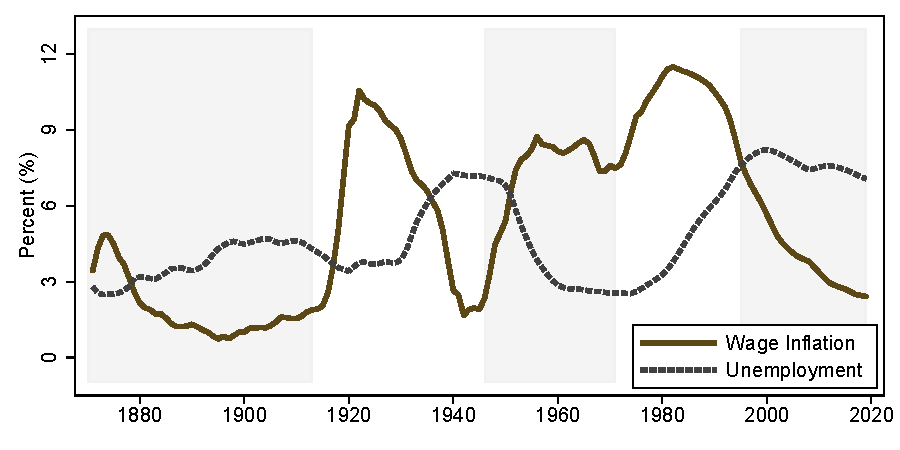
\includegraphics[width=0.9\textwidth]{../Output/Figures/Median_dwn_unemp_paper.pdf}
    \annote{\footnotesize This figure plots a time-varying estimate of the mean wage inflation (solid line) and mean unemployment rate (dashed line) using a 20-year rolling window and the fully matched sample.}
    \label{F_median}
\end{figure}

Summing up, Figure \ref{F_median} points to a strong negative co-movement between the two variables, which is also corroborated at the country level (see Table \ref{T_Correlation} in the Appendix). Nevertheless, during the Gold Standard and the last twenty years, wage inflation and unemployment series were more stable, suggesting a weaker co-movement and thus, unveiling a potentially time-varying wage inflation-unemployment tradeoff. 

In the Appendix, Figure \ref{F_median_country} presents the same exercise for each country using the full sample. Despite the level differences, evidence that motivates the use of country-fixed effects in my regression analysis, the pattern does not uncover a specific country driving the statistics and supports the evidence provided in Figure 1 of a negative co-movement between wage inflation and unemployment, even at the country level.

\subsection{Historical Wage Phillips Curves}

To give more structure to the previous exploratory analysis, I turn my attention to the wage Phillips curve across historical periods. I depart from the wage Phillips curve derived from the micro-founded New Keynesian model presented in \cite{Gali2011}, which I extend to a panel dimension in Appendix \ref{S_Theory}, and estimate the following Equation:

\begin{Equation} \label{EQ:Baseline}
    \pi_{c,t}^w = \mu_c + \varphi u_{c,t} + \gamma \pi_{c,t-1}^p + \epsilon_{c,t}
\end{Equation}

where $\pi_{c,t}^w$ denotes the annual wage inflation in the country $c$ at time $t$; $\alpha$ is a constant; $u_{c,t}$ denotes the unemployment rate in the country $c$ at time $t$; $\pi_{c,t-1}^p$ is the lagged price inflation, the measure by which wages are indexed; and $\epsilon_{c,t}$ is an error term proxying for time-varying cost-push shocks to wages.\footnote{The majority of the literature argues for the use of the unemployment gap instead of its level. However, that approach ignores the problem of measurement error arising from the computation of a natural unemployment rate. In my setting, due to the use of historical data, I believe that the latter poses a bigger threat because it is not possible to use detailed data to get the best estimates of the natural unemployment rate.} The twist of exploring the Phillips curve using a panel approach has been recently explored by \cite{Coibion2019}, \cite{Levy2019}, \cite{DeSchryder2020}, and \cite{Hazell2021} at both national and regional levels. Following the empirical literature, I include time-invariant country fixed effects $\mu_c$. %to account for different local trends. %but do not add year fixed effects.

Here, I implicitly assume that, when there is no reoptimization, wages are indexed to ($\pi_{c,t-1}^p$), where $\gamma$ represents the degree of indexation on past price inflation.\footnote{Another possible interpretation is that firms look at the previous period's price inflation as a good measure of inflation expectations, which then affects their decision in changing both their products' prices and workers' wages.} Given an increase in the price level in $t-1$, workers bargain for a higher wage in $t$ due to an increase in the cost of living in $t-1$.\footnote{Table A.3 in the online Appendix corroborates this idea by displaying a correlation between price inflation in $t-1$ and wage inflation in $t$ of more than 0.5 for almost every country.}

Figure \ref{F:RWIV} shows the time-varying estimates of its slope $(\varphi)$ based on the Panel-OLS regression of Equation \eqref{EQ:Baseline} using a 20-year rolling window. The estimates support the \textit{low inflation hypothesis} which proposes that the slope of the wage Phillips curve is significantly flatter following periods of low price inflation.


\begin{figure}[h]
    \centering
    \caption{Panel-OLS 20-year Rolling Window}
    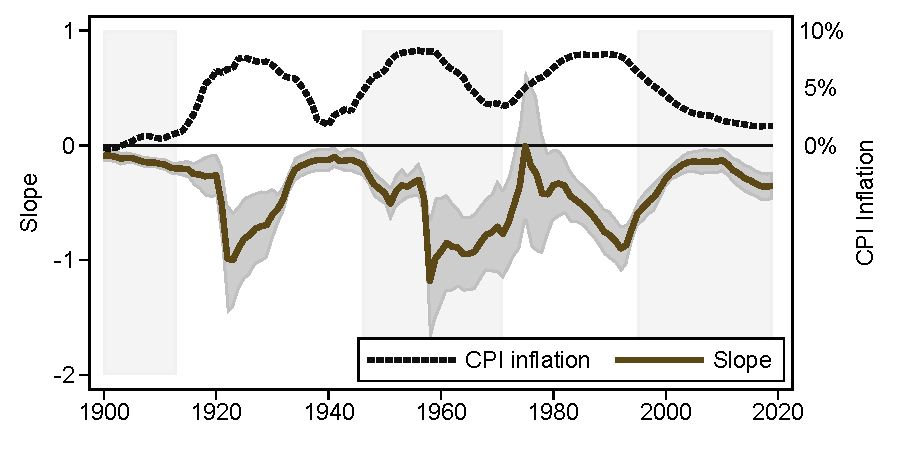
\includegraphics[scale=1]{../Output/Figures/RW_dwn_OLS}
    \annote{\footnotesize This figure plots a time-varying estimate of the slope of the wage Phillips curve (parameter $\varphi$, in Equation \eqref{EQ:Baseline}), using OLS and annual data from 1870 to 2019 for all 18 countries. It is computed based on a rolling OLS regression using a 20-year window and displays a 90\% confidence band. In the Appendix, Figure \ref{F:RWIV_gamma} shows the estimate for the persistence coefficient ($\gamma$); Figure \ref{F:RWIV2} presents the same regression when adding year fixed effects; and Figure \ref{F:RWIV3} presents a population-weighted version of this same graph.}
    \label{F:RWIV}
\end{figure}

There are three key features from Figure \ref{F:RWIV} which deserve to be highlighted. First, it displays the consecutive steepening and flattening of the wage Phillips curve after the end of the Bretton Woods agreement. This pattern is already well documented, especially for the US \citep{Ball2011, Blanchard2015, Blanchard2016, Gali2019} and Europe \citep{Bonam2021}. However, the fact that I am using a panel of 18 advanced economies to perform this analysis might indicate that this flattening could be considered a global phenomenon.

Second, the wage Phillips curve was also flatter during the Gold Standard period and the beginning of the Bretton Woods epoch. This novel finding suggests that the recent weakening of the wage inflation-unemployment tradeoff is not a unique feature of the last 20 years.

Third, it seems that during periods of low price inflation, the slope of the wage Phillips curve becomes flatter. One potential explanation for this correlation is the \textit{low inflation hypothesis} which will be tested in Section \ref{S_Results}. During the majority of the three periods shaded in gray, inflation was being targeted either to the price of gold or to a composite price measure (CPI), and thus, countries experienced a persistent low price inflation environment (as we saw in Table \ref{T:Descriptives}). Consequently, firms adjusted prices and wages less often \citep{Gagnon2009, Nakamura2018, Alvarez2019} and promoted a disconnect between wage inflation and movements in the labor market.\footnote{For a more detailed and analytical explanation, check Appendix \ref{SS_FPA}.}

A major element of modern Phillips curve estimations is \textit{inflation expectations}. \cite{Hazell2021} show that not accounting for the decline in long-run inflation expectations during the Volcker disinflation may introduce an upward bias in estimates of the slope of the United States (price) Phillips curve during that period. Taking this into account might question the use of \cite{Gali2011} framework that may be overly restrictive on the nonexistent role of inflation expectations. Moreover, even though this work focuses only on the relationship between wage inflation and unemployment, it is still important to acknowledge that there is a strong correlation between price and wage inflation (Table \ref{T_Correlation}) and therefore it might be important to have this issue into account. While the absence of historical data on inflation expectations makes it impossible to add it as a control variable, I collect OECD data on inflation forecasts starting in the 1990s for the European countries and starting in the 1960s for the remaining ones to 2019 and run the same analysis for this sub-sample.

Empirically, \cite{Ciccarelli2010} have estimated a common factor in countries' price inflation that accounts for nearly 70\% of their variance. They include 22 OECD countries in their sample - the 18 countries in my sample plus Austria, Greece, Luxembourg, and New Zealand - from 1960 to 2008. With this in mind, it seems worthwhile to include time fixed effects as a way to control not only for the dynamics of global inflation but also to control for the common component (across countries) of inflation expectations.

Figure \ref{F:RWIV2} in the Appendix thus presents the estimates when including year fixed effects or inflation forecast from OECD. It is important to emphasize the difference in the slope estimates from 1990 to 2000 might be due to differences in the sample as most European countries only have expectations data starting in 1991. Not surprisingly, the confidence bands become wider. Notwithstanding, the three key features highlighted before are shown to be robust.

This Section thus provides sufficient and robust \textit{motivation} to explore the time-varying tradeoff between wage inflation and unemployment in more detail while using a more appropriate econometric method.

%\clearpage

\section{Empirical Strategy \label{SS_Identification}}

The literature has extensively documented the empirical challenges in estimating both the price and wage Phillips curves \citep{Gali2011, Mavroeidis2014, Mcleay2019} and, more generally, the wage inflation-unemployment tradeoff which is at the center of this work \citep{Barnichon2019, Gali2019}. The main concern is the simultaneity bias arising from the correlation between the measures of economic slack and inflation with the error term. Departing from an AS-AD model framework, cost-push shocks might affect both the dependent and independent variables. These might be either shocks to input prices such as imported goods, oil, and other important commodities, or input quantities such as a freeze in raw materials production or even wars that drain the labor force. 

\cite{Mcleay2019} made the case that the empirical disconnect between inflation and economic slack is expected to be emphasized when monetary policy is set optimally. Even absent supply shocks, a pure inflation-targeting central bank would neutralize any aggregate demand fluctuations to achieve constant inflation at its target. Hence, inducing a negative correlation between price inflation and economic slack and making it harder to uncover the true relationship between them. It is worth noting, however, that the wage inflation-unemployment tradeoff is less prone to this later criticism because many central banks do not explicitly target the unemployment rate. This observation is undeniably true for the majority of the sample in this study in which only two central banks (the United States and Australia) started targeting unemployment in recent decades.
 
Acknowledging these issues, I use monetary policy shocks to identify the wage inflation-unemployment tradeoff in the same spirit as \cite{Jorda2018}. To be precise, I apply the trilemma IV, a strategy pioneered by \cite{DiGiovanni2009} and recently applied by \cite{Jorda2019} and \cite{Schularick2020}. This allows taking advantage of the fact that economies with fixed exchange rates and under perfect capital mobility are unable to implement independent monetary policies. %\footnote{Another possibility would be using the current and lagged level of real government purchases of goods and services as an instrument \citep{Roberts1995, Barnichon2020}.}

When a country pegs its exchange rate, its interest rate from then on has to closely follow that of the base country; otherwise, there will be unsustainable capital outflows. Moreover, since changes in the base country's interest rate are mainly determined by the base country's economic conditions, their variation is exogenous to the economic conditions in the pegged countries. Notwithstanding, in order to isolate unpredictable movements in the base country's interest rates $\Delta r_b$, I also subtract the predicted changes in the base country's interest rate $\Delta \hat{r}_b$.\footnote{To predict $\Delta \hat{r}_b$, I follow \cite{Jorda2019} and use the first lags of the growth rates of GDP, consumption, investment, stock prices, and credit (all CPI deflated), as well as changes in nominal long-term interest rates, nominal short-term interest rates, the CPI inflation rate, and the current account-to-GDP ratio.}

The trilemma IV, $z_{c,t}$, for local policy rate changes, $\Delta r_{c,t}$, can only be computed when a country's exchange rate is fixed ($\text{Peg}_{c,t}=1$) with respect to a base country $b$ and is thus defined as follows:

\begin{Equation} \label{EQ:trilemmaIV}
	z_{c,t} \equiv (\Delta r_{b(c,t),t} - \Delta \hat{r}_{b(c,t),t}) \times k_{c,t} \times \text{Peg}_{c,t}
\end{Equation}

where $c$ and $t$ are the country and year indices, respectively; $b(c,t)$ denotes country $c$'s base country in year $t$; $\Delta r_{b(c,t),t} - \Delta \hat{r}_{b(c,t),t}$ can be interpreted as a Taylor residual of the base country $b(c,t)$; $\text{Peg}_{c,t}$ takes thew value of 1 if the country is in a fixed exchange rate regime against base country $b$; and $k_{c,t}$ is the degree of capital openness from \cite{Quinn2011}, this index ranges from 0 to 1, with 0 indicating a low degree and 1 a high degree of capital mobility. Both studies by \cite{Jorda2019} and \cite{Schularick2020} show that the trilemma IV is relevant due to its strong relation with changes in pegs' domestic short-term interest rates. In my sample, the instrument exhibits a statistically significant coefficient of 0.65 over the full sample (SE $=0.08$) and for both the pre and post-World War II periods, with the slope coefficients being approximately 0.64 (SE $=0.15$) and 0.65 (SE$=0.09$), respectively (see Table \ref{T:First_Stage} in the Appendix for more details).

Another main challenge that persists even after correcting for endogeneity is specification uncertainty. One can think of estimating a non-parametric version of the Phillips curve without the straitjacket of any ad-hoc functional relation between inflation and economic slack \citep{Gali2019}. Inspired by the fiscal multiplier literature \citep{Ramey2018}, \cite{Barnichon2019} proposed estimating a Phillips multiplier defined as the expected cumulative change in inflation caused by a demand shock that affects expected cumulative unemployment. This statistic directly captures the central bank's inflation-unemployment tradeoff across different horizons, which is consistent with the definition of \cite{Mankiw2001}.

In the following section, I start by tracing the effect of a one percentage point surprise increase in policy rates on average wage inflation and average unemployment rate. To be precise, I estimate impulse response functions (IRFs) by making use of a panel local projections instrumental variable (Panel LP-IV) approach \citep{Jorda2005, Stock2018} as follows:

\begin{Equation} \label{EQ:IRF}
	\bar{X}_{c,t:t+h} = \alpha^X_{c,h} + \beta_h^X z_{c,t} + \zeta^X_h W_{c,t} + e^X_{c,t+h}
\end{Equation}

where $\bar{X}_{c,t:t+h} \equiv \frac{1}{h} \sum^h_{j=0} X_{c,t+j}$ is either the average value of wage inflation or the unemployment rate over $[t,t+h]$, $\alpha^X_{c,h}$ denotes country fixed effects, $z_{c,t}$ is the trilemma IV as introduced in Equation \eqref{EQ:trilemmaIV}, and $W_{c,t}$ is a vector of controls including the world GDP growth and two lags of wage inflation and unemployment.\footnote{Please note for later reference that I include a global real GDP growth variable to parsimoniously remove global business cycle effects as including time-fixed effects would require over a hundred additional parameter estimates.} To remove potential extreme values, throughout the analysis I remove the war periods and observations for which yearly wage inflation is above 50\%.\footnote{Alternatively, I trimmed the first and last percentiles of wage inflation and the results go through.}

Building on these IRFs, I estimate the Phillips multiplier as in \cite{Barnichon2019}. The Phillips multiplier ($\mathcal{P}_h$) can be estimated using a Panel LP-IV approach from the following cumulative regression:

\begin{Equation} \label{EQ:MULT}
	\sum_{j=0}^{h} \pi_{c,t+j}^{w} = \alpha_{c,h} + \mathcal{P}_h \sum_{j=0}^{h} \hat{u}_{c,t+j} + \zeta_h \vec{W}_{c,t} + \epsilon_{c,t+h}
\end{Equation}

where $\alpha_{c,h}$ denotes country fixed effects; $\vec{W}_{c,t}$ is the same vector of control variables as in Equation \eqref{EQ:IRF}; and $\sum_{j=0}^{h} \hat{u}_{c,t+j}$ is instrumented by the trilemma IV, $z_{c,t}$, the exogenous changes in the short-term interest rate in country $c$. These monetary shocks are orthogonal to supply shocks and to the natural unemployment rate under the common assumption that monetary policy is neutral under flexible prices \citep{Gali2015}. Through this IV approach, the Phillips multiplier allows estimating the tradeoff without bias from confounding supply shocks and without the need to measure the natural unemployment rate.

Intuitively, the Phillips multiplier, $\mathcal{P}_h$, measures the impact of a policy that induces a 1 percentage point increase in unemployment on cumulative wage inflation. A negative multiplier ($\mathcal{P}_h < 0$) indicates that a transitory increase in unemployment yields a persistent wage inflation decrease. In other words, central banks can trigger a persistent change in wage inflation at a finite unemployment cost through a transitory increase in their policy interest rates, which is exactly the type of tradeoff monetary policymakers want to explore.

The impulse response functions from Equation \eqref{EQ:IRF} are estimated in such a way that we can obtain the Phillips multiplier directly from $\mathcal{P}_h \equiv \dfrac{\beta_h^{\pi^w}}{\beta_h^{u}}$. The advantage of doing the one-step estimation of the Phillips multiplier in Equation \eqref{EQ:MULT} is to directly obtain the correct confidence bands. Nevertheless, the two-step estimation is consistent once the samples are matched \citep{Ramey2018}.

%\clearpage

\section{Results \label{S_Results}}

Can central banks ``transform" unemployment into inflation (and vice-versa) through their policy interest rates? And, if so, is this tradeoff time-varying and undermined by a low price inflation environment? This section presents the answers provided by the empirical results. I begin by reporting that the central bank's ability to control inflation depends on the unemployment cost of reducing inflation and that its ability is high when considering the full sample. In a second step, I uncover that this ability is impaired when the economy is in a low price inflation environment displaying a different multiplier for two different sub-samples when using long-run annual data and even when zooming in the 1995-2020 period with quarterly data.

\subsection{Phillips multiplier}

Figure \ref{F:Multiplie} displays my estimate for the Phillips multiplier over a 10-year horizon (Figure \ref{F:Multiplier_M}), its F-statistic (Figure \ref{F:Multiplier_F}), and the underlying impulse responses for the average unemployment rate and average wage inflation (Figure \ref{F:Dynamics}). The statistic is initially undetermined, decreasing over the horizon, and becomes significantly negative after 5 years, diverging further on. A 1 percentage point (p.p.) policy-induced increase in cumulative unemployment leads to a 1.4 p.p. decrease in cumulative wage inflation 10 years after the shock.\footnote{In the short-term, the multiplier cannot be interpreted because the value of one of the impulse responses is very close to zero. The uncertainty in the estimation is in line with what \cite{Barnichon2019} also report.}

\begin{figure}[h!]
    \centering
	\caption{Phillips multiplier and IRFs}
	\label{F:Multiplie}
	\begin{subfigure}[b]{0.45\textwidth}
		\caption{Phillips multiplier}
		\label{F:Multiplier_M}
		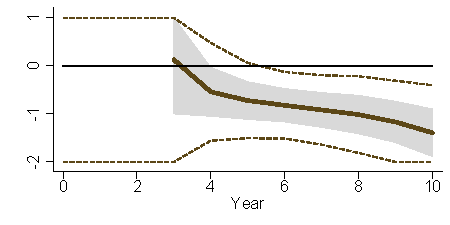
\includegraphics[width=\textwidth]{../Output/Figures/fig_full_PMBM_LPIV10_2.pdf}	
	\end{subfigure}
	\begin{subfigure}[b]{0.45\textwidth}
		\caption{F-Statistic}
		\label{F:Multiplier_F}
		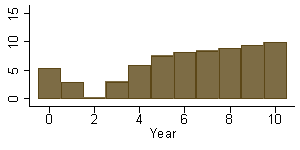
\includegraphics[width=\textwidth]{../Output/Figures/fig_full_PMBM_F_LPIV10_2.pdf}
	\end{subfigure}
	\begin{subfigure}[b]{0.9\textwidth}
		\caption{Impulse Responses}
		\label{F:Dynamics}
		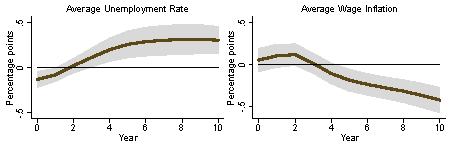
\includegraphics[width=\textwidth]{../Output/Figures/fig_full_LPIVBM10_2.pdf}
		\end{subfigure}
		\annote{Phillips multiplier estimations using the trilemma IV as an instrument, using a matched sample of approximately 800 observations, and controlling for two lags of unemployment and wage inflation, country fixed effects, and world GDP growth as explained in Equation \eqref{EQ:MULT}. For the multiplier (upper-left), the shaded area corresponds to the 90\% confidence interval implied by the normal limiting distribution of the 2SLS estimator, while the dashed lines correspond to the two-sided 90\% Anderson-Rubin confidence sets robust to weak instruments. The F-statistics (upper-right) are computed using the method presented in \cite{Olea2013}. The impulse responses (bottom panels) for \textit{average} wage inflation and \textit{average} unemployment are obtained from the OLS regressions \eqref{EQ:IRF} and display 90\% confidence sets. Impulse responses for non-averaged cumulative unemployment and wage inflation can be found in Figure \ref{F:Non_Avg_Response}.}
	
\end{figure}

As \cite{Barnichon2019} noted, a large tradeoff in the long run implies that a transitory policy-induced change in unemployment has a persistent effect on wage inflation. Hence, Figure \ref{F:Multiplier_M} suggests that, over the last 170 years, central banks had a substantial ability to steer inflation.

Figure \ref{F:Multiplier_F} reports the \cite{Olea2013} F-statistics from the first-stage regression of Equation \eqref{EQ:MULT} and documents that monetary policy shocks are correlated with cumulative unemployment. Since the F-statistic estimates are not above the threshold of \cite{Olea2013} but are still above 5 for most periods, I rely on weak instrument robust methods to compute the confidence bands of the Phillips multiplier. I compute 90\% \cite{Anderson1949} confidence bands that are robust to weak instruments and display them in dashed lines in Figure \ref{F:Multiplier_M}.\footnote{While the asymptotic distribution of the AR statistic does not depend on the strength of the instrument, the confidence bands of the Phillips multiplier will be larger when the instrument is weaker.}

Figure \ref{F:Dynamics} decomposes the Phillips multiplier into the response of both the average wage inflation and the average unemployment rate to a monetary policy surprise. While the average unemployment response starts mean-reverting after horizon $t=5$, the average wage inflation cumulative response decreases persistently. This implies that after the shock, the Phillips multiplier keeps decreasing over time and there is an exploitable tradeoff between unemployment and wage inflation.

%\footnote{For a more complete analysis, Figure \ref{F:IRFs_JST} reports the impulse responses on the rates differentials instead of their averages.}

%\clearpage

\subsection{Smaller Phillips multiplier in low price inflation environments}

Building on the previous Phillips multiplier analysis, I can test whether the wage inflation-unemployment tradeoff is different across sub-samples and, in particular, weaker in times of low price inflation. The baseline specification is thus augmented to include an interaction term. I this estimate a state-dependent Phillips multiplier as follows:

\begin{Equation} \label{EQ:MULT_State}
\begin{split}
	\sum_{j=0}^{h} \pi_{c,t+j}^{w} = & \mathcal{I}_{c,t} \Bigg[\alpha_{c,h}^{(\mathcal{I})} + \mathcal{P}^{(\mathcal{I})}_h \sum_{j=0}^{h} \hat{u}_{c,t+j} + \zeta^{(\mathcal{I})}_h \vec{W}_{c,t}\Bigg] \\  
	& + (1 - \mathcal{I}_{c,t}) \Bigg[\alpha_{c,h}^{(1-\mathcal{I})} + \mathcal{P}^{(1-\mathcal{I})}_h \sum_{j=0}^{h} \hat{u}_{c,t+j} + \zeta^{(1-\mathcal{I})}_h \vec{W}_{c,t}\Bigg] +  \epsilon_{c,t+h}
\end{split}
\end{Equation}

where $\mathcal{I}_{c,t}$ is the indicator variable. This exercise allows comparing the evolution of the Phillips multiplier in each sub-sample and directly test whether $\mathcal{P}_h^{(\mathcal{I})} = \mathcal{P}_h^{(1 - \mathcal{I})}$.

Research on the wage inflation-unemployment tradeoff, traditionally inferred from a Phillips curve, pointed to the hypothesis that  an increase (decrease) in trend inflation should lead to an increase (decrease) in the frequency of price adjustment, thereby decreasing (increasing) the steepness of the wage Phillips curve \citep{Benati2007}.

In this exercise, I test whether the wage inflation-unemployment tradeoff is shaped by a low price inflation environment. Therefore, I estimate Equation \eqref{EQ:MULT_State} where $\mathcal{I}_{c,t}$ is an indicator of low price inflation defined as a dummy variable, which is equal to one for periods when countries experienced lagged price inflation below the threshold of 2\% and above -2\% ($\mathcal{I}_{c,t} = 1 \hspace{1ex} \text{if} \hspace{1ex} -2\% < \pi^p_{c,t-1} < 2\%$) and equal to 0 when countries experienced high price inflation ($\mathcal{I}_{c,t} = 0 \hspace{1ex} \text{if} \hspace{1ex} 2\% \leq \pi^p_{c,t-1} < 40\%$). This exercise allows comparing the evolution of the Phillips multiplier in times of low versus high price inflation and directly test whether $\mathcal{P}_h^{(\mathcal{I})} = \mathcal{P}_h^{(1-\mathcal{I})}$.

The choice of the 2\% threshold can be rationalized by the inflation target strategy of many of the central banks present in the analyzed sample. Over the last 20 years of the sample, most central banks were targeting inflation either implicitly or explicitly (Table \ref{T_HistoricalPeriodsSource1}). Most of them disclaimed that their goal was to achieve inflation close to or below 2\%. With such a sample division, I am assigning 75\% of the sample to the high-inflation state and 25\% to the low price inflation state as summarized in Figure \ref{F:Sample_SD}.

Figure \ref{F2:Multiplier} displays the estimates of both the baseline and state-dependent Phillips multipliers over a 10-year horizon (Figure \ref{F2:Multiplier_M}), their F-statistics (Figure \ref{F2:Multiplier_F}), and their underlying average impulse responses (Figure \ref{F2:Dynamics}) in periods of high and low price inflation.

\begin{figure}[h!]
    \centering
	\caption{State-Dependent Phillips multiplier and IRFs}
	\label{F2:Multiplier}
	\begin{subfigure}[b]{0.45\textwidth}
		\caption{Phillips multiplier}
		\label{F2:Multiplier_M}
		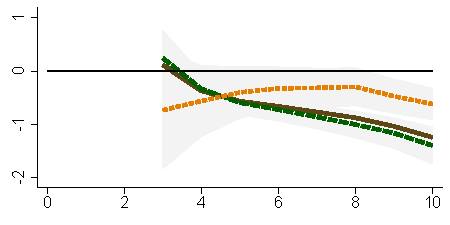
\includegraphics[width=\textwidth]{../Output/Figures/fig_full_SDPMBM_LPIV10_2_asym_lowflat.pdf}	
	\end{subfigure}
	\begin{subfigure}[b]{0.45\textwidth}
		\caption{F-Statistic}
		\label{F2:Multiplier_F}
		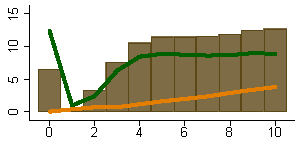
\includegraphics[width=\textwidth]{../Output/Figures/fig_full_PMBM_F_LPIV10_2_asym_lowflat.pdf}
	\end{subfigure}
	\begin{subfigure}[b]{0.9\textwidth}
		\caption{Impulse Responses}
		\label{F2:Dynamics}
		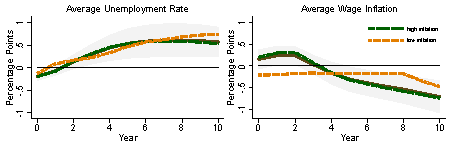
\includegraphics[width=\textwidth]{../Output/Figures/fig_full_SDLPIVBM10_2_asym_lowflat.pdf}
		\end{subfigure}
		\annote{Phillips multiplier estimated using the trilemma IV as instrument according to Equation \eqref{EQ:MULT}. For each state-multiplier (upper-left), the shaded areas correspond to the 90\% confidence interval implied by the normal limiting distribution of the 2SLS estimator. The F-statistics (upper-right) are computed as discussed in \cite{Olea2013}. The impulse responses (bottom panels) for \textit{average} wage inflation and unemployment are obtained from the OLS regressions \eqref{EQ:IRF} and display 90\% confidence sets for the baseline estimate. Across all figures, one can distinguish the state by its color and line pattern: orange and short-dashed for low inflation; green and long-dashed for high inflation.}
	
\end{figure}

Figure \ref{F2:Multiplier_M} displays a smaller Phillips multiplier in times of low inflation and a higher multiplier in times of high inflation. Its difference becomes statistically significant from horizon $t=8$ onward with the weak instrument robust Anderson-Rubin p-values being 0.070, 0.076, and 0.056 for horizons 8, 9, and 10 respectively. This result is in line with recent work by, among others, \cite{Forbes2021} who show that the Phillips curve becomes non-linear and flatter when inflation is low. Table \ref{T:SDPM} in the Appendix presents a detailed description of this result displaying the point estimates, their standard errors, and the weak instrument robust Anderson-Rubin p-values for testing the difference in multipliers across states.

Figure \ref{F2:Dynamics} indicates that the wage inflation response is the main driver of the weaker tradeoff in low inflation periods. Although the average unemployment rate response is virtually identical in both the baseline and the state dependencies for longer horizons, the average wage inflation response is much flatter during low inflation periods. 

As a robustness check, I also used an unmatched sample and a longer horizon (see Figure \ref{F:Multiplier_SD_App} and Table \ref{T:SDPM_App} in the Appendix). Regardless of the chosen sample trimming process or horizon, the wage inflation-unemployment tradeoff is weaker in a low price inflation environment.

These two exercises together lend empirical substance to the concern that monetary policy effects are time-variant and state-dependent. In particular, during periods of low price inflation, the long-run tradeoff between wage inflation and unemployment is less exploitable. In other words, given the weaker tradeoff, central banks are less able to steer wage inflation when facing a low price inflation environment.

\subsection{Low price inflation or monetary policy regime?}

The previous exercise presents evidence consistent with the key message of this paper: the Phillips multiplier is smaller when monetary policy is implemented following periods of low inflation (Figure \ref{F2:Multiplier}).

Notwithstanding, this exercise does not allow us to distinguish whether the state-dependent effects of monetary policy for different inflation environments (low or high) are driven by different sample periods. That is because different sample periods could capture different monetary policy regimes and hence different multipliers.

To be more precise on the low inflation mechanism I put forward, I first run a robustness check where I account for different monetary policy regimes. I then conduct a thorough analysis using quarterly frequency data since 1995 for 17 out of 18 countries in the baseline sample, evaluating whether \textit{within} the same monetary policy regime the low inflation motive is still present.

The first exercise has the goal of capturing structural differences that are common across countries in the same monetary policy regimes. I start by identifying different monetary policy regimes as described in Appendix \ref{SS_HistoricalPeriods} and summarized in Table \ref{T_HistoricalPeriodsSource1}. I then add different monetary policy regime dummies when estimating Equations \eqref{EQ:MULT} and \eqref{EQ:MULT_State} which differ across countries according to Table \ref{T_HistoricalPeriodsSource1}. I do so for the following regimes: Gold Standard; Interwar and Bretton Woods; and Implicit Inflation Targeting. When doing so, the number of estimated coefficients increases and thus, the uncertainty around the estimates also increases. Nevertheless, Table \ref{T:SDPM_MP} qualitatively corroborates the key finding of the paper: when monetary policy is implemented in periods of low inflation, the tradeoff between wage inflation and unemployment is weaker.

\paragraph{Addressing external validity by focusing on one monetary policy regime and using higher frequency data.}

For the second exercise, I compiled information for 17 out of 18 countries, excluding Switzerland, from the Federal Reserve Economic Data (FRED) at the quarter level since 1995. Then, I estimated Equation \eqref{EQ:MULT}, using the non-residualized version of the instrument defined by Equation \eqref{EQ:trilemmaIV}, keeping the same horizon of 10 years (40 quarters) and using a matched sample.

In many ways, this exercise is a replication of \cite{Barnichon2019} based on their Proposition 1 (Equation 4) and differing in three dimensions. First, I am analyzing a panel of countries in a fixed exchange rate regime instead of the United States and the United Kingdom separately. Second, I based my identification on the trilemma of international finance instead of narrative identification to characterize monetary policy shocks. Finally, my sample is based on the period between 1995q1 and 2019q4, incorporating the Great Recession Period but excluding the Covid pandemic. Like \cite{Barnichon2019}, I use quarterly data, include four lags of inflation and unemployment as control variables, and rely on weak instrument robust methods for computing the confidence sets for the Phillips multiplier \citep{Anderson1949}.

In Appendix, Figure \ref{F:MultiplierQ} replicates Figure \ref{F:Multiplie} using this quarterly data. Compared to the baseline, Figure \ref{F:MultiplierQ} displays a smaller multiplier and a much weaker average wage inflation response. This latter finding is in accordance with the exercise where \cite{Barnichon2019} split their sample and focus on the post-1990 sample period (Figures 4 and 6).

%F-statistic being small The asymptotic distribution of the Anderson-Rubin confidence sets does not depend on the strength of the instrument, however, the confidence bands of the Phillips multiplier are larger when the instruments are weaker \cite{Barnichon2019}.  

To go one step further, I then test whether the Phillips multiplier is weaker in periods of low inflation using this quarterly sample. I thus estimate Equation \eqref{EQ:MULT_State}. Figure \ref{F:MultiplierQ_SD} presents the results.

\begin{figure}[h!]
    \centering 
	\caption{Phillips multiplier and IRFs}
	\label{F:MultiplierQ_SD}
	\begin{subfigure}[b]{0.45\textwidth}
		\caption{Phillips multiplier}
		\label{F:MultiplierQ_SD_M}
		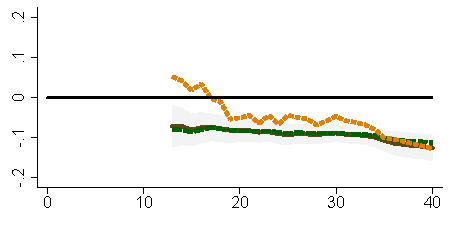
\includegraphics[width=\textwidth]{../Output/Figures/fig_full_SDPMBM_LPIV40_2_asym_lowflat_Quarter.pdf}	
	\end{subfigure}
	\begin{subfigure}[b]{0.45\textwidth}
		\caption{F-Statistic}
		\label{F:MultiplierQ_SD_F}
		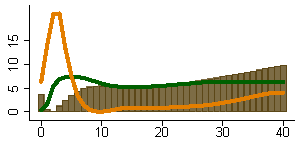
\includegraphics[width=\textwidth]{../Output/Figures/fig_full_PMBM_F_LPIV40_2_asym_lowflat_Quarter.pdf}
	\end{subfigure}
	\begin{subfigure}[b]{0.9\textwidth}
		\caption{Impulse Responses}
		\label{F:DynamicsQ_SD}
		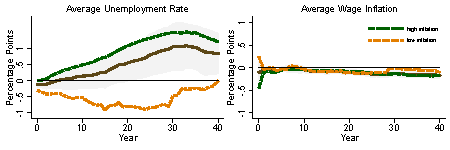
\includegraphics[width=\textwidth]{../Output/Figures/fig_full_SDLPIVBM40_2_asym_lowflat_Quarter.pdf}
		\end{subfigure}
		\annote{Phillips multiplier estimations using the trilemma IV as an instrument, using a matched sample of 465 quarterly observations between 1995q1 and 2019q4, and controlling for two lags of unemployment and wage inflation, country fixed effects, and world GDP growth as explained in Equation \eqref{EQ:MULT} but now at the quarterly frequency. 230 (235) observations are assigned to high (low) inflation environments following the proposed classification. For each state-multiplier (upper-left), the shaded areas correspond to the 90\% confidence interval implied by the normal limiting distribution of the 2SLS estimator which overlap. The F-statistics (upper-right) are computed using the method presented in \cite{Olea2013}. The impulse responses (bottom panels) for \textit{average} wage inflation and \textit{average} unemployment are obtained from the OLS regressions \eqref{EQ:IRF} and display 90\% confidence sets for the linear estimate.}
	
\end{figure}

The weak instrument robust Anderson-Rubin p-values for the difference in the high versus low price inflation multipliers are presented in Table \ref{T:SDPM_Q} together with the point estimates of Figure \ref{F:MultiplierQ_SD_F} and their standard errors. Even using such a limited sample, focusing on the period between 1995q1 and 2019q4, and with quarterly level data, we are still able to find that the wage inflation-unemployment tradeoff is weaker during periods of low price inflation.

I still find a statistically significantly weaker multiplier during a low price inflation episode and for some horizons. But, interestingly enough, for a different reason. While Figure \ref{F:Multiplier_SD} tells us that it is the muted wage inflation response driving the weaker multiplier, Figure \ref{F:MultiplierQ_SD} tells us that since 1995 the stronger unemployment response is actually driving the weaker multiplier.


\section{Conclusion \label{S_Conclusion}}
 
The wage inflation-unemployment tradeoff is a key building block for monetary policy. This paper introduces newly assembled data on wages and unemployment rates for a set of 18 advanced economies starting in 1870, in order to revisit the historical relationship between wage inflation and unemployment, the focus of Phillips' (\citeyear{Phillips1958}) original work. The empirical analysis starts by uncovering a historical time-varying Phillips correlation. This paper documents a weaker correlation between wage inflation and unemployment in a low price inflation environment.

I capitalize on the assembled historical data to study a factor that is possibly driving this time-varying pattern. First, in order to account for the possible endogeneity and model misspecification issues arising from the Phillips curve framework, I make use of monetary policy shocks and the Phillips multiplier framework to identify the historical wage inflation-unemployment tradeoff. The results provide evidence in favor of the hypothesis that the tradeoff is weaker in periods of low price inflation.

These results add a new perspective to the current debate about the existence of the wage inflation-unemployment tradeoff and its state dependency. In particular, this paper's empirical evidence points to an impaired ability in exploring the tradeoff in times of low inflation driven by a stronger unemployment rate and a muted wage inflation response to a monetary policy surprise. 

%Such a finding uncovers a hidden dichotomy: central banks cannot simultaneously target a low price inflation (2\%) and expect conventional monetary policy tools to work to their full extent.

\clearpage

\begin{singlespace}
\bibliographystyle{chicago}
\bibliography{Bibliography}   
\end{singlespace}


\clearpage

\begin{appendices}

\setcounter{page}{1}
\setcounter{table}{0}
\setcounter{figure}{0}
\renewcommand{\thepage}{\roman{page}}
\renewcommand{\thetable}{\Alph{section}.\arabic{table}}
\renewcommand{\thefigure}{\Alph{section}.\arabic{figure}}
\renewcommand{\theEquation}{\Alph{section}.\arabic{Equation}}

\begin{titlepage}

\begin{center}
\textbf{\huge{Monetary Policy and the Wage \\ Inflation-Unemployment Tradeoff}}\\

\vspace{2em}

\textbf{\huge{Online Appendix}}\\

\vspace{2em}

\textbf{\Large{Ricardo Duque Gabriel \\ University of Bonn}}\\
\end{center}

\thispagestyle{empty}
%\maketitle

\end{titlepage}

\section{Supporting tables and figures}


\begin{table}[ht]
\caption{Data Coverage}
\label{T_DataCoverage}
\centering
\def\sym#1{\ifmmode^{#1}\else\(^{#1}\)\fi}
\begin{tabular}{l*{4}{c}}
\hline\hline
\textbf{Country}    & \textbf{Wages}  & \textbf{Unemployment} & \textbf{Inflation Forecast} & \textbf{CB Foundation} \\
\hline
Australia       & 1870-2019 & 1901-2019 & 1961-2019 & 1911\\
Belgium         & 1870-2019 & 1921-2019 & 1992-2019 & 1850\\
Canada          & 1870-2019 & 1916-2019 & 1993-2019 & 1934\\
Denmark         & 1870-2019 & 1874-2019 & 1968-2019 & 1818\\
Finland         & 1870-2019 & 1920-2019 & 1991-2019 & 1811\\
France          & 1870-2019 & 1895-2019 & 1991-2019 & 1800\\
Germany         & 1870-2019 & 1887-2019 & 1996-2019 & 1876\\
Ireland			& 1943-2019 & 1960-2019 & 1996-2019 & 1943\\
Italy           & 1871-2019 & 1919-2019 & 1991-2019 & 1893\\
Japan           & 1870-2019 & 1930-2019 & 1961-2019 & 1882\\
Netherlands     & 1870-2019 & 1870-2019 & 1991-2019 & 1814\\
Norway          & 1870-2019 & 1904-2019 & 1961-2019 & 1816\\
Portugal        & 1870-2019 & 1953-2019 & 1991-2019 & 1846\\
Spain           & 1870-2019 & 1933-2019 & 1993-2019 & 1874\\
Sweden          & 1870-2019 & 1911-2019 & 1963-2019 & 1668\\
Switzerland     & 1870-2019 & 1913-2019 & 1963-2019 & 1907\\
United Kingdom  & 1870-2019 & 1870-2019 & 1991-2019 & 1694\\
United States   & 1870-2019 & 1890-2019 & 1961-2019 & 1913\\
\hline\hline
\end{tabular}
\annote{\footnotesize This Table shows the earliest and the latest data point for each country's series used in this paper: the wages nominal index and the unemployment rate. The updated data series are available on \href{https://www.ricardoduquegabriel.com/publication/gabriel_2020_hwpc/}{my website}. There are gaps in the unemployment rate data which mostly correspond to the war periods, for more information on the gaps and the sources please consult the Data Appendix. Data from the inflation forecast comes from the OECD. All central bank foundations dates came from the central banks' websites.}
\end{table}

\clearpage

\begin{table}[!h]
\caption{Descriptive statistics - full sample}
\label{T_Descriptives_Full}
\centering
\def\sym#1{\ifmmode^{#1}\else\(^{#1}\)\fi}
\begin{tabular}{l*{1}{ccccc}}
\hline\hline
                    &       \textbf{N}    &        \textbf{Mean}&   \textbf{Std. Dev.}&         \textbf{Min}&         \textbf{Max}\\
\hline
\textbf{1870-1913}           &            &            &            &            &            \\
Unemployment rate   &         225&        4.08&        2.73&        0.20&       18.40\\
Wage inflation      &         730&        1.81&        4.23&      -24.64&       23.80\\
Price inflation     &         731&        0.46&        4.76&      -26.91&       33.31\\
\hline
\textbf{World Wars}          &            &            &            &            &            \\
Unemployment rate   &         130&        3.63&        2.97&        0.40&       17.20\\
Wage inflation      &         213&       14.85&       32.90&      -19.94&      412.23\\
Price inflation     &         228&       20.29&       71.10&      -37.68&      975.64\\
\hline
\textbf{1920-1938 }          &            &            &            &            &            \\
Unemployment rate   &         270&        7.12&        5.00&        0.60&       24.90\\
Wage inflation      &         314&        3.13&       13.16&      -27.72&       86.48\\
Price inflation     &         333&        0.67&        9.84&      -19.42&       73.13\\
\hline
\textbf{1946-1971 }          &            &            &            &            &            \\
Unemployment rate   &         436&        2.60&        1.84&        0.04&        9.92\\
Wage inflation      &         465&       10.11&       19.44&      -55.42&      225.19\\
Price inflation     &         468&        5.38&       10.37&      -17.60&      125.33\\
\hline
\textbf{1972-1999}           &            &            &            &            &            \\
Unemployment rate   &         504&        7.07&        4.30&        0.04&       24.21\\
Wage inflation      &         504&        8.30&        6.27&       -1.42&       32.28\\
Price inflation     &         504&        6.56&        5.51&       -0.71&       37.88\\
\hline
\textbf{2000-2020}           &            &            &            &            &            \\
Unemployment rate   &         377&        7.05&        3.52&        2.00&       26.09\\
Wage inflation      &         378&        2.32&        1.84&       -6.14&        7.50\\
Price inflation     &         378&        1.63&        1.28&       -4.48&        5.57\\
\hline
\textbf{Total}               &            &            &            &            &            \\
Unemployment rate   &        1942&        5.49&        4.08&        0.04&       26.09\\
Wage inflation      &        2604&        5.85&       14.41&      -55.42&      412.23\\
Price inflation     &        2642&        4.40&       22.54&      -37.68&      975.64\\
\hline\hline
\end{tabular}
\annote{\footnotesize All statistics are expressed in percent. The hyperinflation period in Germany (1920-1925) is not included. All remaining observations available in the dataset are used in this Table.}
\end{table}

\clearpage

\begin{table}[htbp]\centering
\def\sym#1{\ifmmode^{#1}\else\(^{#1}\)\fi}
\caption{Descriptive statistics - weighted sample \label{T:DescriptivesW}}
\begin{tabular}{l*{1}{cccccc}}
\hline\hline
                    &\multicolumn{6}{c}{}                                                         \\
                    &       count&         p50&        mean&          sd&         min&         max\\
\hline
1870-1913           &            &            &            &            &            &            \\
Unemployment rate   &         223&        4.00&        4.97&        3.42&        0.20&       18.40\\
Wage inflation      &         223&        1.41&        1.56&        2.14&       -6.71&       10.26\\
Price inflation     &         223&        0.20&        0.51&        2.15&      -10.94&       11.56\\
\hline
1920-1938           &            &            &            &            &            &            \\
Unemployment rate   &         268&        6.30&        8.34&        6.14&        0.60&       24.90\\
Wage inflation      &         268&        0.18&        1.46&        8.40&      -27.72&       43.97\\
Price inflation     &         268&        0.30&        0.04&        6.97&      -18.45&       30.43\\
\hline
1946-1971           &            &            &            &            &            &            \\
Unemployment rate   &         428&        2.73&        3.25&        2.03&        0.04&        9.92\\
Wage inflation      &         428&        6.07&        7.36&        4.92&      -10.78&       35.29\\
Price inflation     &         428&        3.19&        3.91&        3.69&       -6.87&       20.38\\
\hline
1972-1999           &            &            &            &            &            &            \\
Unemployment rate   &         504&        6.20&        6.76&        3.76&        0.04&       24.21\\
Wage inflation      &         504&        4.94&        7.02&        5.87&       -1.42&       32.28\\
Price inflation     &         504&        4.16&        5.57&        4.77&       -0.71&       37.88\\
\hline
2000-2020           &            &            &            &            &            &            \\
Unemployment rate   &         360&        5.78&        6.73&        3.39&        2.00&       26.09\\
Wage inflation      &         360&        2.57&        2.17&        1.72&       -3.49&        7.50\\
Price inflation     &         360&        1.75&        1.67&        1.23&       -4.48&        5.57\\
\hline
Total               &            &            &            &            &            &            \\
Unemployment rate   &        1783&        5.30&        5.99&        4.02&        0.04&       26.09\\
Wage inflation      &        1783&        3.29&        4.69&        5.65&      -27.72&       43.97\\
Price inflation     &        1783&        2.28&        3.10&        4.52&      -18.45&       37.88\\
\hline\hline
\end{tabular}
\end{table}
\annote{\footnotesize All statistics are expressed in percent. The war periods (1914-1919 and 1939-1945) and the German hyperinflation episode (1920-1925) are not included. This table only uses \textit{weighted} by population country-year observations for which there is data for the unemployment rate, and price and wage inflation. Table \ref{T:Descriptives-Full} presents descriptive statistics for the unrestricted sample.}


\clearpage

% matrix: C file: C:\Users\Ricardo\Documents\GitHub\Monetary-Policy-and-the-Wage-Inflation-Unemployment-Tradeoff\Output\Tables\Correlation_Wage_Fix.tex  20 Apr 2023 12:33:23
\begin{table}[htbp]
\caption{\label{T_Correlation} Wage Inflation Correlations Table}\centering\medskip
\begin{tabular}{lccc} \hline \hline
 & $\pi_t^p$  & $\pi_{t-1}^p$  & $\hspace{0em}u_t$  \\  \hline 
Australia &     0.699 &     0.693 &    -0.459 \\  
Belgium &     0.406 &     0.595 &    -0.193 \\  
Canada &     0.807 &     0.497 &    -0.423 \\  
Denmark &     0.657 &     0.673 &    -0.091 \\  
Finland &     0.372 &     0.475 &    -0.353 \\  
France &     0.835 &     0.726 &    -0.514 \\  
Germany &     0.691 &     0.625 &    -0.534 \\  
Italy &     0.635 &     0.772 &    -0.101 \\  
Japan &     0.286 &     0.382 &    -0.749 \\  
Netherlands &     0.628 &     0.581 &    -0.321 \\  
Norway &     0.814 &     0.729 &    -0.626 \\  
Portugal &     0.585 &     0.620 &    -0.234 \\  
Spain &     0.546 &     0.466 &    -0.268 \\  
Sweden &     0.806 &     0.775 &    -0.497 \\  
Switzerland &     0.626 &     0.715 &    -0.482 \\  
UK &     0.762 &     0.574 &    -0.266 \\  
USA &     0.858 &     0.574 &    -0.287 \\  
Ireland &     0.830 &     0.650 &    -0.196 \\  
\hline \hline \end{tabular}
\end{table}
\annote{\footnotesize Correlation between wage inflation and price inflation, lagged price inflation, and unemployment by country in the main sample excluding outliers as defined in the text.}


\begin{table}[ht]
\centering
\caption{First-Stage of trilemma IV} \label{T:First_Stage}
\vspace{1ex}
\def\sym#1{\ifmmode^{#1}\else\(^{#1}\)\fi}
                    &\multicolumn{1}{c}{(1)}&\multicolumn{1}{c}{(2)}&\multicolumn{1}{c}{(3)}&\multicolumn{1}{c}{(4)}&\multicolumn{1}{c}{(5)}&\multicolumn{1}{c}{(6)}\\
                    &\multicolumn{1}{c}{All years}&\multicolumn{1}{c}{PreWW2}&\multicolumn{1}{c}{PostWW2}&\multicolumn{1}{c}{All years}&\multicolumn{1}{c}{PreWW2}&\multicolumn{1}{c}{PostWW2}\\
\hline
JST trilemma instrument (residualized base rate changes)&        0.60\sym{***}&        0.41\sym{***}&        0.68\sym{***}&        0.65\sym{***}&        0.64\sym{***}&        0.64\sym{***}\\
                    &      (0.08)         &      (0.09)         &      (0.09)         &      (0.08)         &      (0.15)         &      (0.09)         \\
[1em]
Constant            &       -0.05\sym{**} &       -0.06\sym{***}&       -0.02         &        0.10         &        0.01         &       -0.06         \\
                    &      (0.02)         &      (0.02)         &      (0.02)         &      (0.10)         &      (0.09)         &      (0.17)         \\
\hline
$ t $-statistic     &      [7.65]         &      [4.42]         &      [7.98]         &      [8.36]         &      [4.29]         &      [7.24]         \\
N                   &        1307         &         505         &         802         &        1002         &         215         &         787         \\

\annote{This table presents the first-stage estimates of the trilemma IV on the country's interest rate. The standard errors are in parentheses and the T-statistics are in square brackets. The full sample covers 1870–2019, excluding the World Wars and the German hyperinflation episode. The pre-WW2 sample covers 1870–1938, excluding 1914–1919, while the post-WW2 sample covers 1948–2019. The estimates in the last three columns (with controls) include country fixed effects and two lags of wage inflation and unemployment rate. In addition, I include world GDP growth to capture global cycles.}
\end{table}

\begin{table}[ht]
\centering
\caption{First-Stage of trilemma IV - Quarterly Data} \label{T:First_Stage_Quarter}
\vspace{1ex}
\def\sym#1{\ifmmode^{#1}\else\(^{#1}\)\fi}
\begin{tabular}{lccc}
\toprule
Dependent & \multicolumn{1}{c}{No controls} && \multicolumn{1}{c}{With controls} \\
variable: $\Delta r_{it}$       \\
\midrule
trilemma $ z_{i,t}$ &   0.89\sym{***} &&   0.67\sym{***}  \\
& (  0.03 ) && (  0.03 )   \\
t-statistic & [30.94] && [21.31] \\
\# Obs &          917 &&          852 \\
\bottomrule
\end{tabular}

\annote{This table presents the first-stage estimates of the trilemma IV on the country's interest rate for quarterly data. The standard errors are in parentheses and the T-statistics are in square brackets. The full sample covers 1995q1–2019q4. The estimates in the last column (with controls) include country-fixed effects and two lags of wage inflation and unemployment rate. In addition, I include world GDP growth to capture global cycles.}
\end{table}

\begin{singlespace}
\begin{table}[ht]
\footnotesize
\centering
\def\sym#1{\ifmmode^{#1}\else\(^{#1}\)\fi}
\caption{Estimates of multipliers across states of inflation \label{T:SDPM}}
\begin{tabular}{l*{1}{cccc}}
\hline\hline
 Horizon  & Linear & High                 & Low           & AR            \\
                  & Model         & Inflation & Inflation & p-value       \\
\hline
   3       & 0.112 & 0.242 & -0.735 & 0.135 \\
          & (0.452) & (0.523) & (1.098) & \\
 & & & &\\
   4       & -0.373 & -0.336 & -0.563 & 0.451 \\
          & (0.256) & (0.285) & (0.668) & \\
 & & & &\\
   5       & -0.565 & -0.593 & -0.402 & 0.775 \\
          & (0.199) & (0.229) & (0.482) & \\
 & & & &\\
   6       & -0.664 & -0.726 & -0.327 & 0.327 \\
          & (0.173) & (0.213) & (0.402) & \\
 & & & &\\
   7       & -0.769 & -0.863 & -0.315 & 0.137 \\
          & (0.171) & (0.223) & (0.369) & \\
 & & & &\\
   8       & -0.878 & -1.003 & -0.296 & 0.070 \\
          & (0.184) & (0.251) & (0.356) & \\
 & & & &\\
   9       & -1.038 & -1.165 & -0.472 & 0.076 \\
          & (0.200) & (0.286) & (0.322) & \\
 & & & &\\
  10       & -1.244 & -1.398 & -0.618 & 0.056 \\
          & (0.230) & (0.346) & (0.299) & \\
 & & & &\\
\hline\hline
\end{tabular}

\annote{\footnotesize This table presents the multiplier estimates corresponding to the ones in Figure \ref{F2:Multiplier_M}. The values in parentheses under the multipliers indicate the corresponding standard errors. The last column indicates the weak instrument robust Anderson-Rubin p-values for the difference in multipliers across states.}
\end{table}

\begin{table}[ht]
\footnotesize
\centering
\def\sym#1{\ifmmode^{#1}\else\(^{#1}\)\fi}
\caption{Estimates of multipliers across states of inflation - unmatched sample \label{T:SDPM_App}}
\begin{tabular}{l*{1}{cccc}}
\hline\hline
 Horizon  & Linear & High                 & Low           & AR            \\
                  & Model         & Inflation & Inflation & p-value       \\
\hline
   3       & -0.041 & 0.285 & -0.677 & 0.137 \\
          & (0.354) & (0.648) & (0.329) & \\
 & & & &\\
   4       & -0.460 & -0.391 & -0.679 & 0.438 \\
          & (0.200) & (0.309) & (0.241) & \\
 & & & &\\
   5       & -0.650 & -0.696 & -0.668 & 0.933 \\
          & (0.162) & (0.241) & (0.237) & \\
 & & & &\\
   6       & -0.760 & -0.830 & -0.719 & 0.709 \\
          & (0.155) & (0.224) & (0.297) & \\
 & & & &\\
   7       & -0.810 & -0.956 & -0.595 & 0.180 \\
          & (0.148) & (0.232) & (0.210) & \\
 & & & &\\
   8       & -0.886 & -1.058 & -0.606 & 0.089 \\
          & (0.165) & (0.254) & (0.248) & \\
 & & & &\\
   9       & -1.004 & -1.177 & -0.571 & 0.051 \\
          & (0.176) & (0.277) & (0.180) & \\
 & & & &\\
  10       & -1.221 & -1.405 & -0.684 & 0.061 \\
          & (0.220) & (0.348) & (0.213) & \\
 & & & &\\
  11       & -1.403 & -1.592 & -0.543 & 0.037 \\
          & (0.270) & (0.410) & (0.344) & \\
 & & & &\\
  12       & -1.474 & -1.671 & -0.598 & 0.049 \\
          & (0.271) & (0.425) & (0.342) & \\
 & & & &\\
  13       & -1.677 & -1.898 & -0.794 & 0.092 \\
          & (0.307) & (0.514) & (0.350) & \\
 & & & &\\
  14       & -1.776 & -1.966 & -0.831 & 0.122 \\
          & (0.337) & (0.545) & (0.344) & \\
 & & & &\\
  15       & -1.918 & -2.096 & -0.724 & 0.119 \\
          & (0.401) & (0.621) & (0.364) & \\
 & & & &\\
\hline\hline
\end{tabular}

\annote{\footnotesize This table presents the multiplier estimates corresponding to the ones in Figure \ref{F2:Multiplier_MM}. The values in parentheses under the multipliers indicate the standard errors. The last column indicates the weak instrument robust Anderson-Rubin p-values for the difference in multipliers across states.}
\end{table}

\begin{table}[ht]
\footnotesize
\centering
\def\sym#1{\ifmmode^{#1}\else\(^{#1}\)\fi}
\caption{Estimates of multipliers across states of inflation - Monetary Policy Regimes \label{T:SDPM_MP}}
\begin{tabular}{l*{1}{cccc}}
\hline\hline
 Horizon  & Linear & High                 & Low           & AR            \\
                  & Model         & Inflation & Inflation & p-value       \\
\hline
   3       & 0.294 & 0.297 & 0.239 & 0.355 \\
          & (0.897) & (0.897) & (3.060) & \\
 & & & &\\
   4       & -0.227 & -0.228 & 0.072 & 0.810 \\
          & (0.432) & (0.486) & (1.154) & \\
 & & & &\\
   5       & -0.370 & -0.418 & 0.078 & 0.675 \\
          & (0.320) & (0.403) & (0.746) & \\
 & & & &\\
   6       & -0.403 & -0.462 & 0.113 & 0.452 \\
          & (0.267) & (0.378) & (0.574) & \\
 & & & &\\
   7       & -0.468 & -0.555 & 0.134 & 0.250 \\
          & (0.252) & (0.379) & (0.520) & \\
 & & & &\\
   8       & -0.569 & -0.716 & 0.148 & 0.129 \\
          & (0.267) & (0.431) & (0.489) & \\
 & & & &\\
   9       & -0.799 & -1.010 & -0.058 & 0.108 \\
          & (0.326) & (0.578) & (0.407) & \\
 & & & &\\
  10       & -1.144 & -1.586 & -0.211 & 0.048 \\
          & (0.472) & (0.992) & (0.345) & \\
 & & & &\\
\hline\hline
\end{tabular}
\annote{\footnotesize This table presents the multiplier estimates when adding monetary policy regime dummies to Equation \eqref{EQ:MULT_State}. The values in parentheses under the multipliers indicate the corresponding standard errors. The last column indicates the weak instrument robust Anderson-Rubin p-values for the difference in multipliers across states.}
\end{table}

\clearpage

\footnotesize{
\centering{
\begin{longtable}{l*{1}{cccc}}
\def\sym#1{\ifmmode^{#1}\else\(^{#1}\)\fi}
\caption{Estimates of multipliers across states of inflation - quarterly data \label{T:SDPM_Q}}
\hline
 Horizon  & Linear & High                 & Low           & AR            \\
                  & Model         & Inflation & Inflation & p-value       \\
\hline
 13       & -0.071 & -0.079 & 0.053 & 0.351 \\
          & (0.032) & (0.031) & (0.176) & \\
 & & & &\\
  14       & -0.072 & -0.081 & 0.042 & 0.207 \\
          & (0.028) & (0.025) & (0.139) & \\
 & & & &\\
  15       & -0.081 & -0.086 & 0.019 & 0.171 \\
          & (0.024) & (0.023) & (0.112) & \\
 & & & &\\
  16       & -0.075 & -0.080 & 0.034 & 0.051 \\
          & (0.023) & (0.023) & (0.122) & \\
 & & & &\\
  17       & -0.074 & -0.075 & -0.003 & 0.161 \\
          & (0.020) & (0.021) & (0.101) & \\
 & & & &\\
  18       & -0.077 & -0.078 & -0.010 & 0.171 \\
          & (0.020) & (0.020) & (0.099) & \\
 & & & &\\
  19       & -0.082 & -0.081 & -0.054 & 0.336 \\
          & (0.018) & (0.018) & (0.080) & \\
 & & & &\\
  20       & -0.082 & -0.083 & -0.051 & 0.295 \\
          & (0.017) & (0.015) & (0.079) & \\
 & & & &\\
  21       & -0.083 & -0.083 & -0.044 & 0.142 \\
          & (0.016) & (0.013) & (0.078) & \\
 & & & &\\
  22       & -0.086 & -0.085 & -0.064 & 0.140 \\
          & (0.015) & (0.012) & (0.065) & \\
 & & & &\\
  23       & -0.085 & -0.083 & -0.044 & 0.027 \\
          & (0.014) & (0.011) & (0.068) & \\
 & & & &\\
  24       & -0.091 & -0.087 & -0.067 & 0.048 \\
          & (0.015) & (0.011) & (0.058) & \\
 & & & &\\
  25       & -0.093 & -0.090 & -0.044 & 0.029 \\
          & (0.015) & (0.010) & (0.063) & \\
 & & & &\\
  26       & -0.090 & -0.087 & -0.050 & 0.040 \\
          & (0.014) & (0.010) & (0.058) & \\
 & & & &\\
  27       & -0.091 & -0.089 & -0.053 & 0.071 \\
          & (0.014) & (0.009) & (0.056) & \\
 & & & &\\
  28       & -0.093 & -0.089 & -0.069 & 0.176 \\
          & (0.014) & (0.009) & (0.051) & \\
 & & & &\\
  29       & -0.090 & -0.088 & -0.058 & 0.124 \\
          & (0.013) & (0.009) & (0.043) & \\
 & & & &\\
  30       & -0.089 & -0.089 & -0.047 & 0.120 \\
          & (0.013) & (0.009) & (0.048) & \\
 & & & &\\
  31       & -0.092 & -0.091 & -0.057 & 0.181 \\
          & (0.013) & (0.009) & (0.043) & \\
 & & & &\\
  32       & -0.093 & -0.092 & -0.062 & 0.173 \\
          & (0.014) & (0.010) & (0.042) & \\
 & & & &\\
  33       & -0.095 & -0.092 & -0.067 & 0.223 \\
          & (0.013) & (0.010) & (0.039) & \\
 & & & &\\
  34       & -0.099 & -0.095 & -0.079 & 0.400 \\
          & (0.014) & (0.010) & (0.037) & \\
 & & & &\\
  35       & -0.107 & -0.100 & -0.100 & 0.719 \\
          & (0.016) & (0.010) & (0.036) & \\
 & & & &\\
  36       & -0.114 & -0.106 & -0.104 & 0.800 \\
          & (0.018) & (0.011) & (0.034) & \\
 & & & &\\
  37       & -0.117 & -0.108 & -0.110 & 0.865 \\
          & (0.018) & (0.012) & (0.036) & \\
 & & & &\\
  38       & -0.120 & -0.110 & -0.115 & 0.952 \\
          & (0.019) & (0.012) & (0.036) & \\
 & & & &\\
  39       & -0.122 & -0.110 & -0.121 & 0.821 \\
          & (0.019) & (0.012) & (0.036) & \\
 & & & &\\
  40       & -0.126 & -0.112 & -0.128 & 0.681 \\
          & (0.019) & (0.013) & (0.036) & \\
 & & & &\\
\hline\hline
\end{longtable}
\annote{\footnotesize This table presents the multiplier estimates when estimating Equation \eqref{EQ:MULT_State} using quarterly data. The values in parentheses under the multipliers indicate the corresponding standard errors. The last column indicates the weak instrument robust Anderson-Rubin p-values for the difference in multipliers across states. Similarly to the yearly exercise, the Table only reports information from year 3 onwards.}
}}

\clearpage

%\begin{figure}[h!]
%	
    %\centering
    %\caption{Impulse Responses}
	%	\label{F:IRFs_JST}
	%	\includegraphics[width=\textwidth]{fig_full_LPIV10_2.pdf}
	%	\annote{This figure plots the impulse responses for the changes in the wage inflation rate (right panel) and unemployment rate (left panel) which are obtained from OLS regressions close to \eqref{EQ:IRF} but with $\bar{X}_{c,t:t+h} \equiv X_{c,t+j} - X_{c,t-1}$, where $X$ can be either the wage inflation rate or the unemployment rate \textbf{instead of averaged values}. 90\% confidence bounds are displayed.}
%\end{figure}


\begin{figure}[ht]
    \centering
    \caption{Wage inflation (solid) and unemployment rate (dash) across countries} \label{F_median_country}
    \begin{subfigure}[b]{0.30\textwidth}
    \caption*{Australia}
    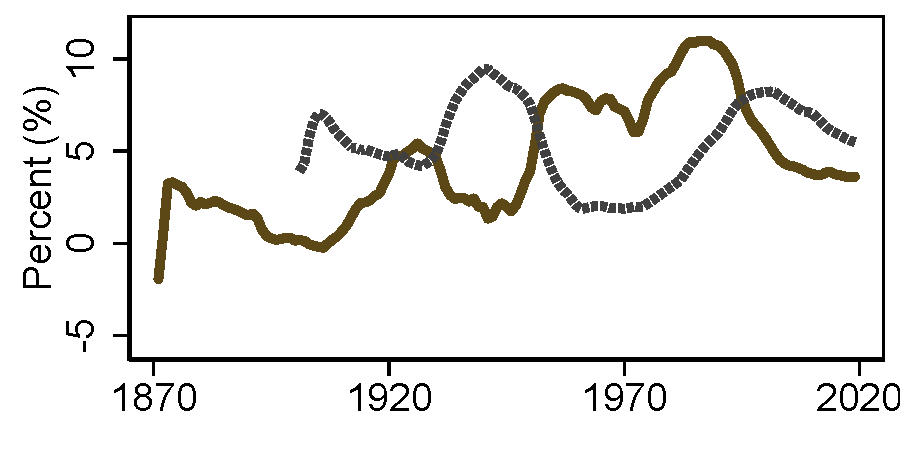
\includegraphics[width=\textwidth]{../Output/Figures/Median_dwn_unemp_Australia.pdf}   
    \end{subfigure}
    \begin{subfigure}[b]{0.30\textwidth}
    \caption*{Belgium}
    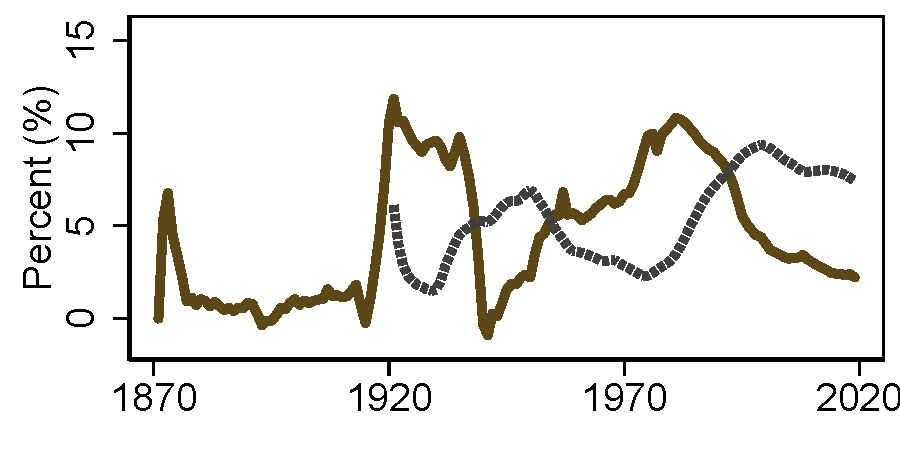
\includegraphics[width=\textwidth]{../Output/Figures/Median_dwn_unemp_Belgium.pdf}   
    \end{subfigure}
    \begin{subfigure}[b]{0.30\textwidth}
    \caption*{Canada}
    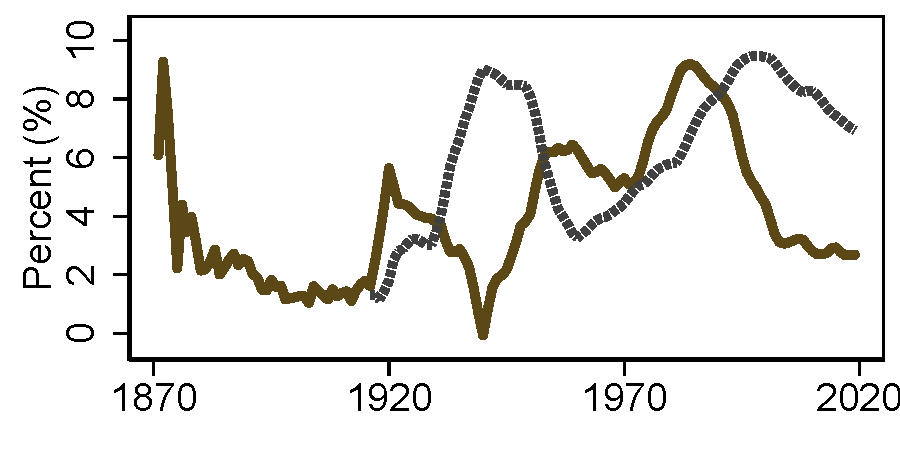
\includegraphics[width=\textwidth]{../Output/Figures/Median_dwn_unemp_Canada.pdf}   
    \end{subfigure} 
    \begin{subfigure}[b]{0.30\textwidth}
    \caption*{Denmark}
    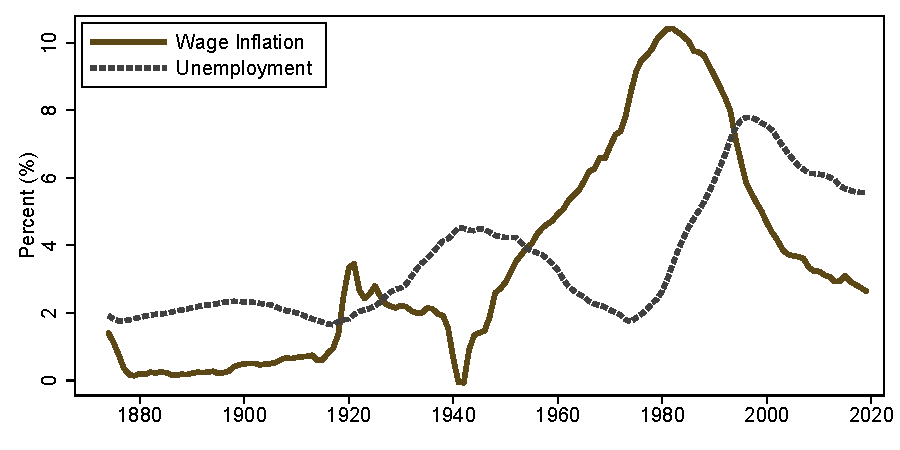
\includegraphics[width=\textwidth]{../Output/Figures/Median_dwn_unemp_Denmark.pdf}   
    \end{subfigure} 
    \begin{subfigure}[b]{0.30\textwidth}
    \caption*{Finland}
    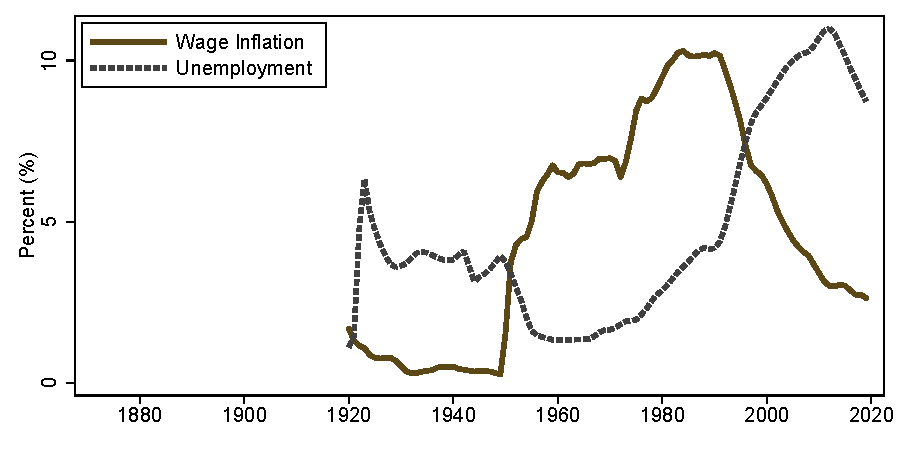
\includegraphics[width=\textwidth]{../Output/Figures/Median_dwn_unemp_Finland.pdf}   
    \end{subfigure}
    \begin{subfigure}[b]{0.30\textwidth}
    \caption*{France}
    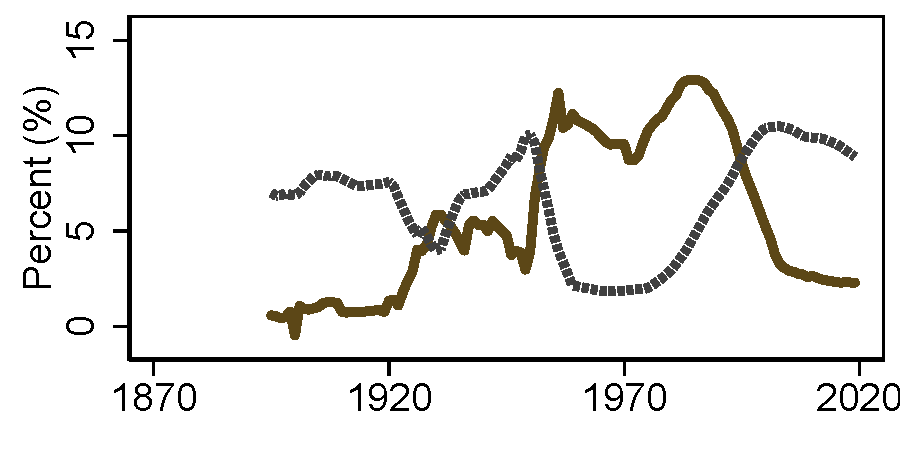
\includegraphics[width=\textwidth]{../Output/Figures/Median_dwn_unemp_France.pdf}   
    \end{subfigure}
    \begin{subfigure}[b]{0.30\textwidth}
    \caption*{Germany}
    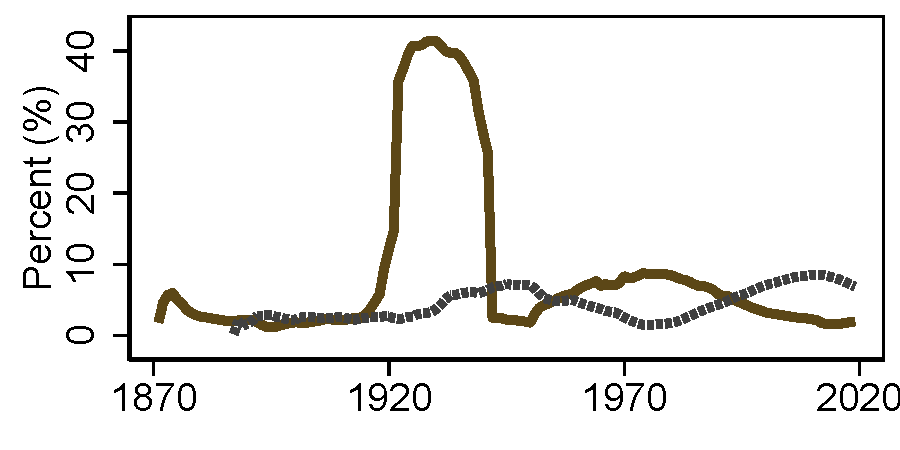
\includegraphics[width=\textwidth]{../Output/Figures/Median_dwn_unemp_Germany.pdf}   
    \end{subfigure} 
    \begin{subfigure}[b]{0.30\textwidth}
    \caption*{Ireland}
    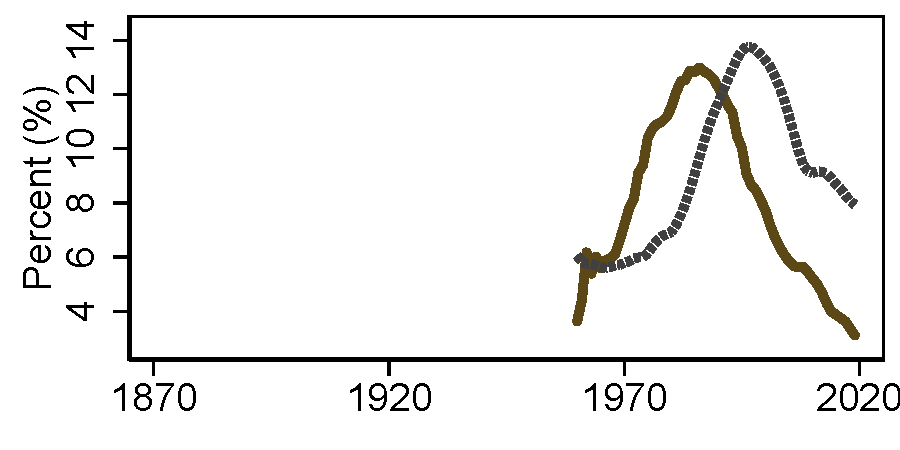
\includegraphics[width=\textwidth]{../Output/Figures/Median_dwn_unemp_Ireland.pdf}   
    \end{subfigure} 
    \begin{subfigure}[b]{0.30\textwidth}
    \caption*{Italy}
    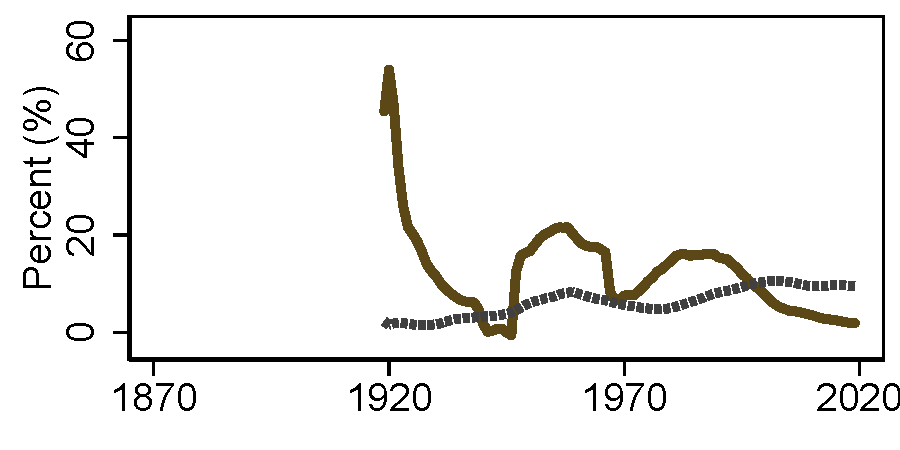
\includegraphics[width=\textwidth]{../Output/Figures/Median_dwn_unemp_Italy.pdf}   
    \end{subfigure}
    \begin{subfigure}[b]{0.30\textwidth}
    \caption*{Japan}
    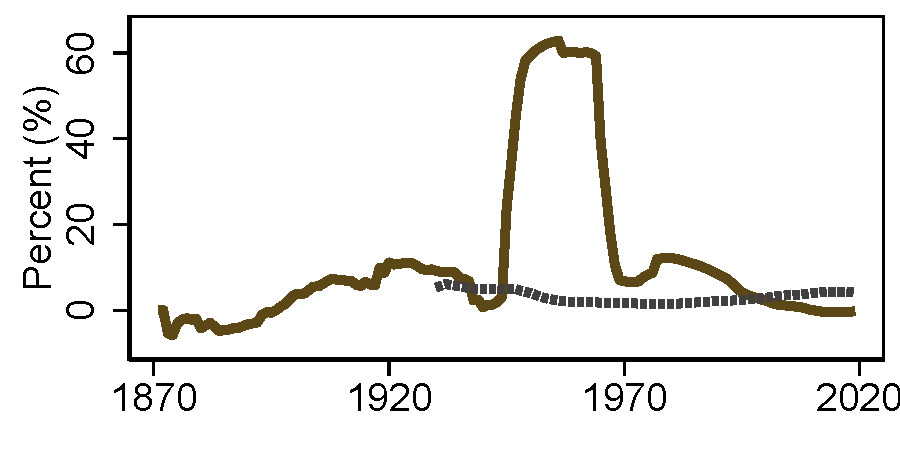
\includegraphics[width=\textwidth]{../Output/Figures/Median_dwn_unemp_Japan.pdf}   
    \end{subfigure}
    \begin{subfigure}[b]{0.30\textwidth}
    \caption*{Netherlands}
    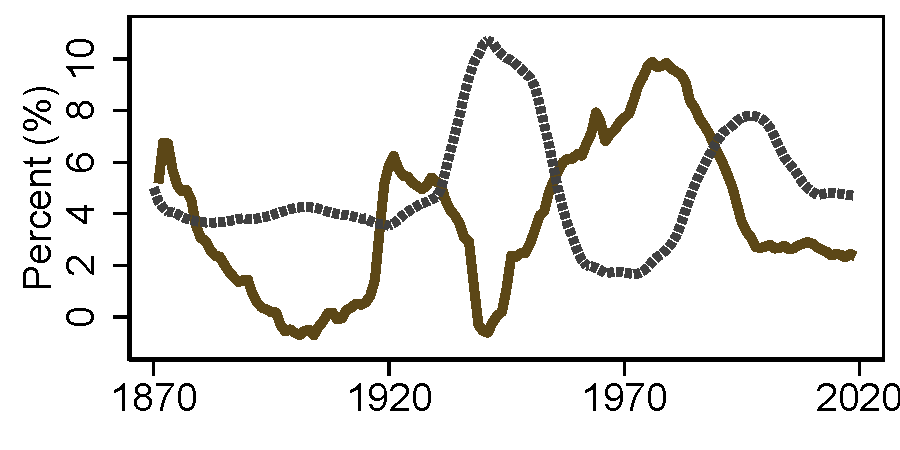
\includegraphics[width=\textwidth]{../Output/Figures/Median_dwn_unemp_Netherlands.pdf}   
    \end{subfigure} 
    \begin{subfigure}[b]{0.30\textwidth}
    \caption*{Norway}
    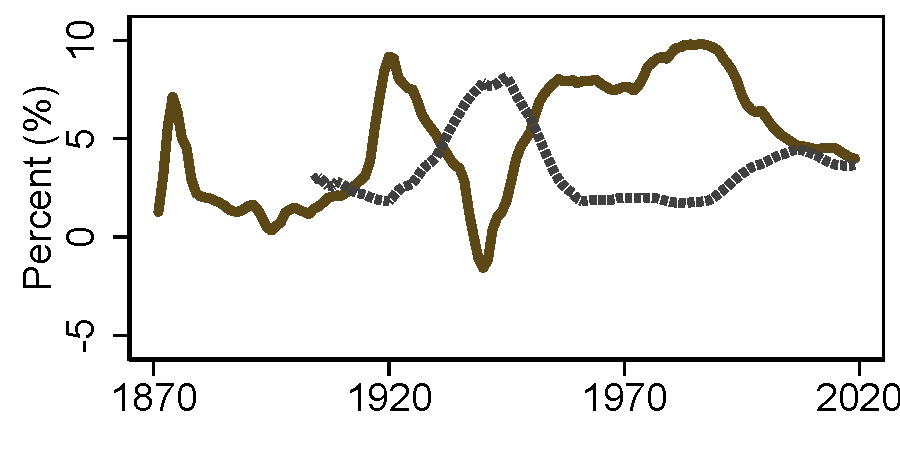
\includegraphics[width=\textwidth]{../Output/Figures/Median_dwn_unemp_Norway.pdf}   
    \end{subfigure} 
    \begin{subfigure}[b]{0.30\textwidth}
    \caption*{Portugal}
    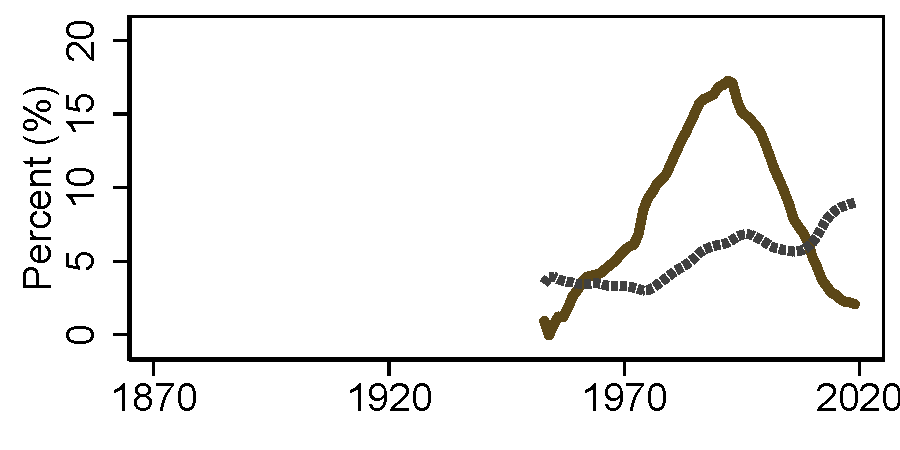
\includegraphics[width=\textwidth]{../Output/Figures/Median_dwn_unemp_Portugal.pdf}   
    \end{subfigure}
    \begin{subfigure}[b]{0.30\textwidth}
    \caption*{Spain}
    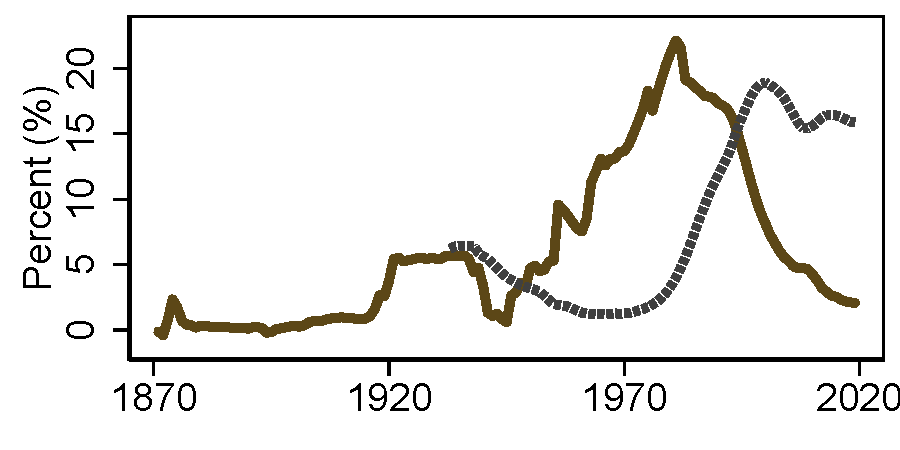
\includegraphics[width=\textwidth]{../Output/Figures/Median_dwn_unemp_Spain.pdf}   
    \end{subfigure}
    \begin{subfigure}[b]{0.30\textwidth}
    \caption*{Sweden}
    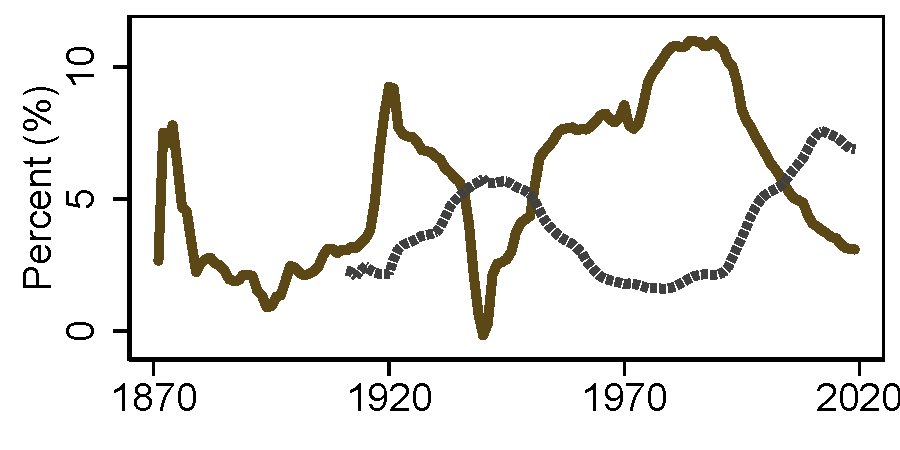
\includegraphics[width=\textwidth]{../Output/Figures/Median_dwn_unemp_Sweden.pdf}   
    \end{subfigure} 
    \begin{subfigure}[b]{0.30\textwidth}
    \caption*{Switzerland}
    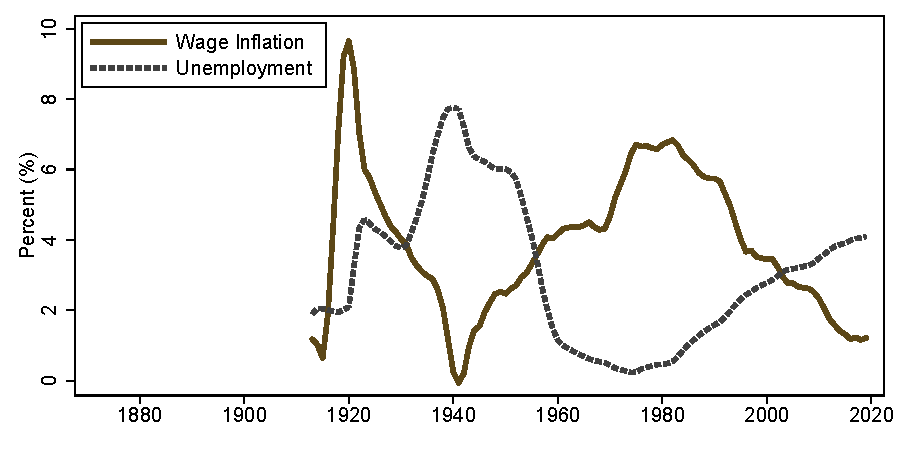
\includegraphics[width=\textwidth]{../Output/Figures/Median_dwn_unemp_Switzerland.pdf}   
    \end{subfigure} 
    \begin{subfigure}[b]{0.30\textwidth}
    \caption*{United Kingdom}
    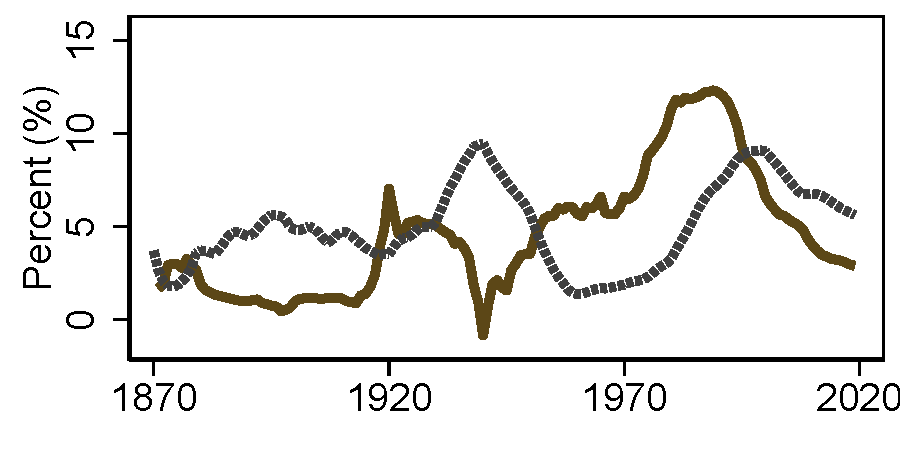
\includegraphics[width=\textwidth]{../Output/Figures/Median_dwn_unemp_UK.pdf}   
    \end{subfigure}
    \begin{subfigure}[b]{0.30\textwidth}
    \caption*{United States}
    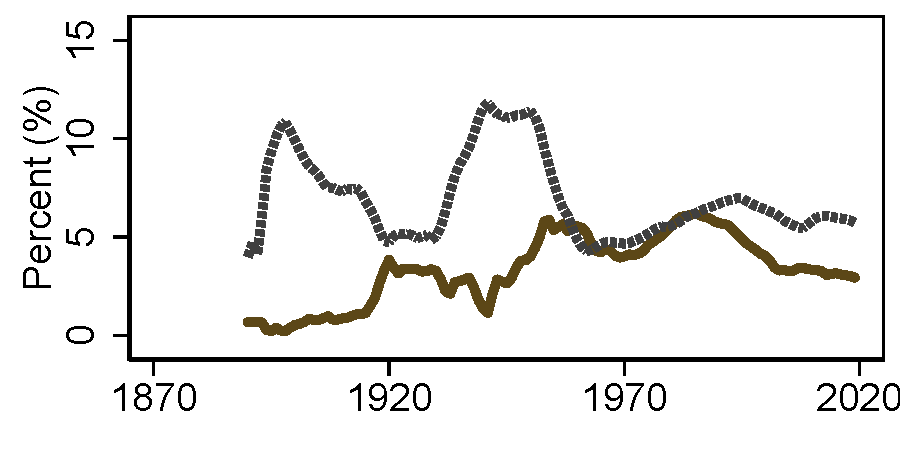
\includegraphics[width=\textwidth]{../Output/Figures/Median_dwn_unemp_USA.pdf}   
    \end{subfigure} 
    \annote{\footnotesize These figures plot a time-varying estimate of the mean wage inflation (solid line) and mean unemployment rate (dashed line) using a 20-year rolling window for each country.}
\end{figure}


\begin{figure}[h!]
    \centering
    \caption{Panel-OLS 20-year Rolling Window}
    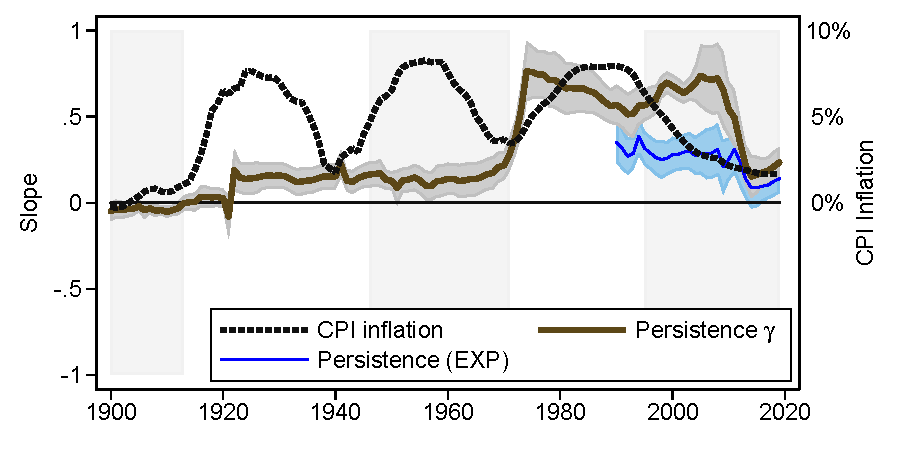
\includegraphics[scale=0.9]{../Output/Figures/RW_cpi_OLS}
    \annote{\footnotesize This figure plots a time-varying estimate of the persistence coefficient of the wage Phillips curve (parameter $\gamma$, in Equation \eqref{EQ:Baseline}), using OLS and annual data from 1870 to 2019 for all 18 countries. In blue, I estimate the parameter $\gamma$ also controling for inflation expectations by estimating: $\pi_{c,t}^w = \mu_c + \pi_{t+1}^e + \varphi u_{c,t} + \gamma \pi_{c,t-1}^p + \epsilon_{c,t}$. It is computed based on a rolling OLS regression using a 20-year window and displays a 90\% confidence band.}
    \label{F:RWIV_gamma}
\end{figure}

\begin{figure}[h!]
    \centering
    \caption{Panel-OLS 20-year Rolling Window with year fixed effects}
    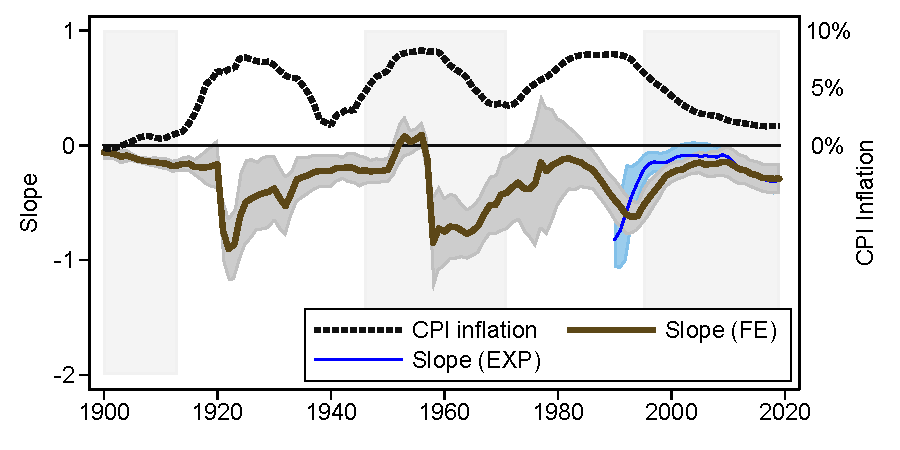
\includegraphics[scale=0.9]{../Output/Figures/RW_dwn_OLS_year}
    \annote{\footnotesize This figure plots a time-varying estimate of the slope of the wage Phillips curve for two different specifications of Equation \eqref{EQ:Baseline}. In brown, I estimate the parameter $\varphi$  by estimating: $\pi_{c,t}^w = \mu_c + \delta_t + \varphi u_{c,t} + \gamma \pi_{c,t-1}^p + \epsilon_{c,t}$. In blue, I estimate the parameter $\varphi$  by estimating: $\pi_{c,t}^w = \mu_c + \pi_{t+1}^e + \varphi u_{c,t} + \gamma \pi_{c,t-1}^p + \epsilon_{c,t}$. In both specifications I am using Panel-OLS and annual data from 1870 to 2019 for all 18 countries. It is computed based on a rolling OLS regression using a 20-year window with year fixed effects ($\delta_t$) and displays a 90\% confidence band.}
    \label{F:RWIV2}
\end{figure}

\begin{figure}[h!]
    \centering
    \caption{Panel-OLS 20-year weighted Rolling Window}
    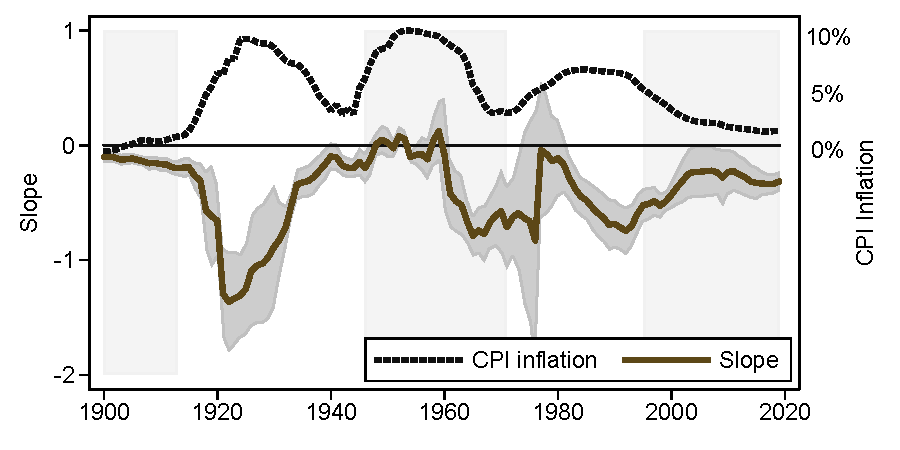
\includegraphics[scale=0.9]{../Output/Figures/RW_dwn_OLS_w}
    \annote{\footnotesize This figure plots a time-varying estimate of the slope of the wage Phillips curve for a weighted version of Equation \eqref{EQ:Baseline}. I am using Panel-OLS and annual data from 1870 to 2019 for all 18 countries. It is computed based on a rolling OLS regression using a 20-year window weighted by population size. It displays a 90\% confidence band.}
    \label{F:RWIV3}
\end{figure}

\begin{figure}[h!]
    \centering
    \caption{Impulse Responses of Cumulative Changes in Unemployment and Wage Inflation}
	\label{F:Non_Avg_Response}
	\begin{subfigure}[b]{0.75\textwidth}
		\includegraphics[width=\textwidth]{../Output/Figures/fig_full_LPIV10_2.pdf}
	\end{subfigure}
\annote{These impulse responses for cumulative unemployment and cumulative wage inflation are obtained from the OLS regressions \eqref{EQ:IRF} by changing the dependent variable from the average $\dfrac{1}{h} \sum^h_{j=0} y_{c,t+j}$ to the difference $y_{c,t+j}-y_{c,t-1}$. They display 90\% confidence sets and show the temporary effect of the monetary policy shock to unemployment and the persistent effect to the wage inflation (in line with the persistent effect to price inflation in \cite{Jorda2019}).}
\end{figure}

\begin{figure}[h!]
    \centering
    \caption{Sample composition for Phillips multiplier estimation}
    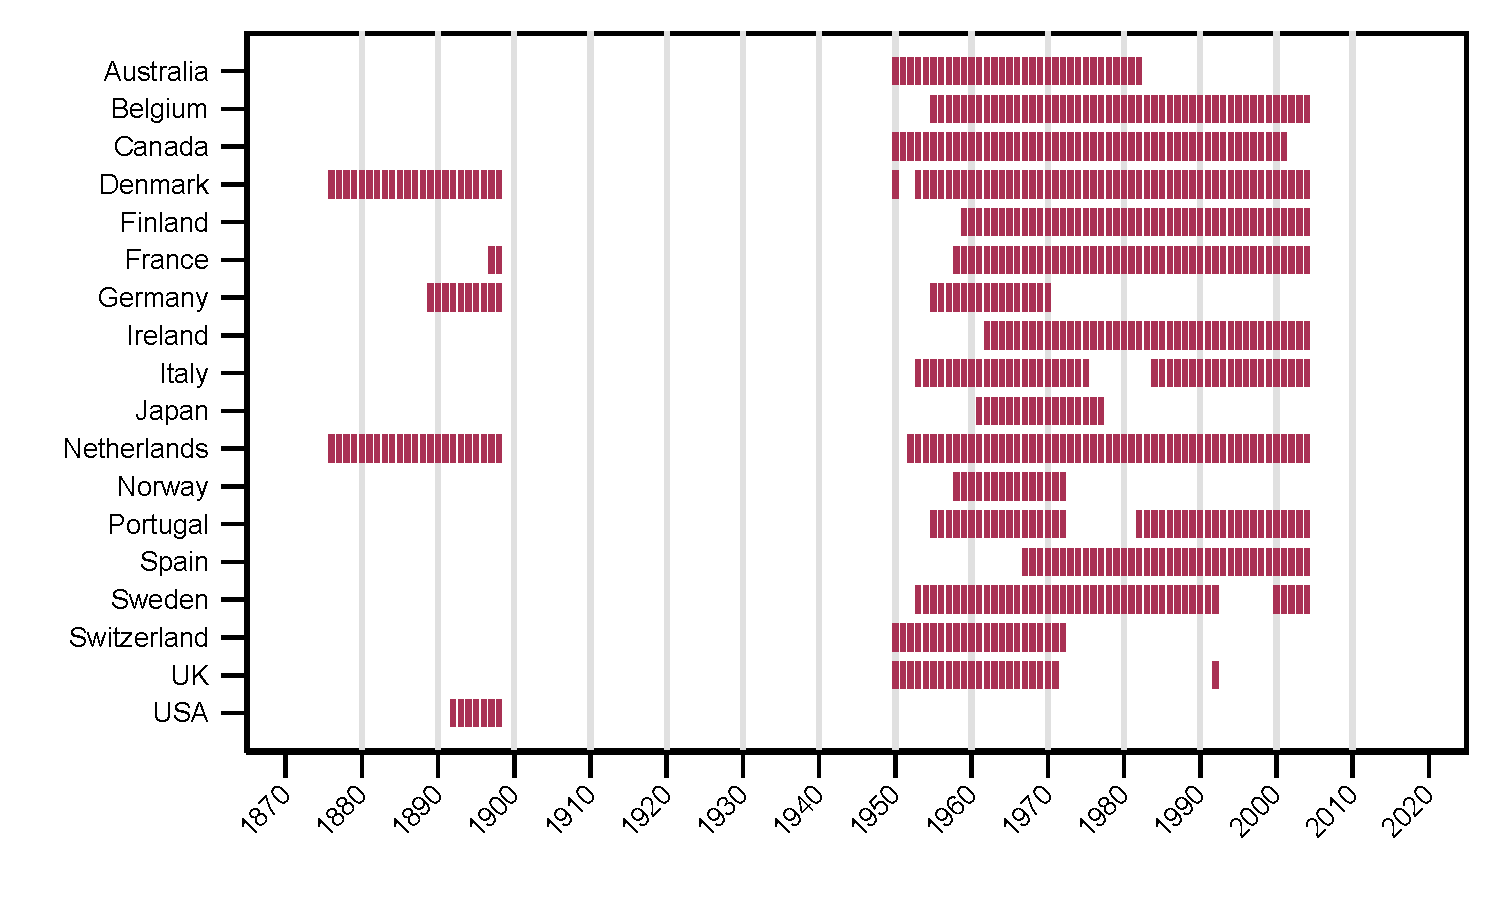
\includegraphics[scale=0.55]{../Output/Figures/history_Sample}
    \annote{\footnotesize This figure displays which year-country observations are being used when estimating the Phillips multiplier for the matched sample.}
    \label{F:Sample}
\end{figure}

\begin{figure}[h!]
    \centering
    \caption{Sample composition for state-dependent Phillips multiplier estimation}
    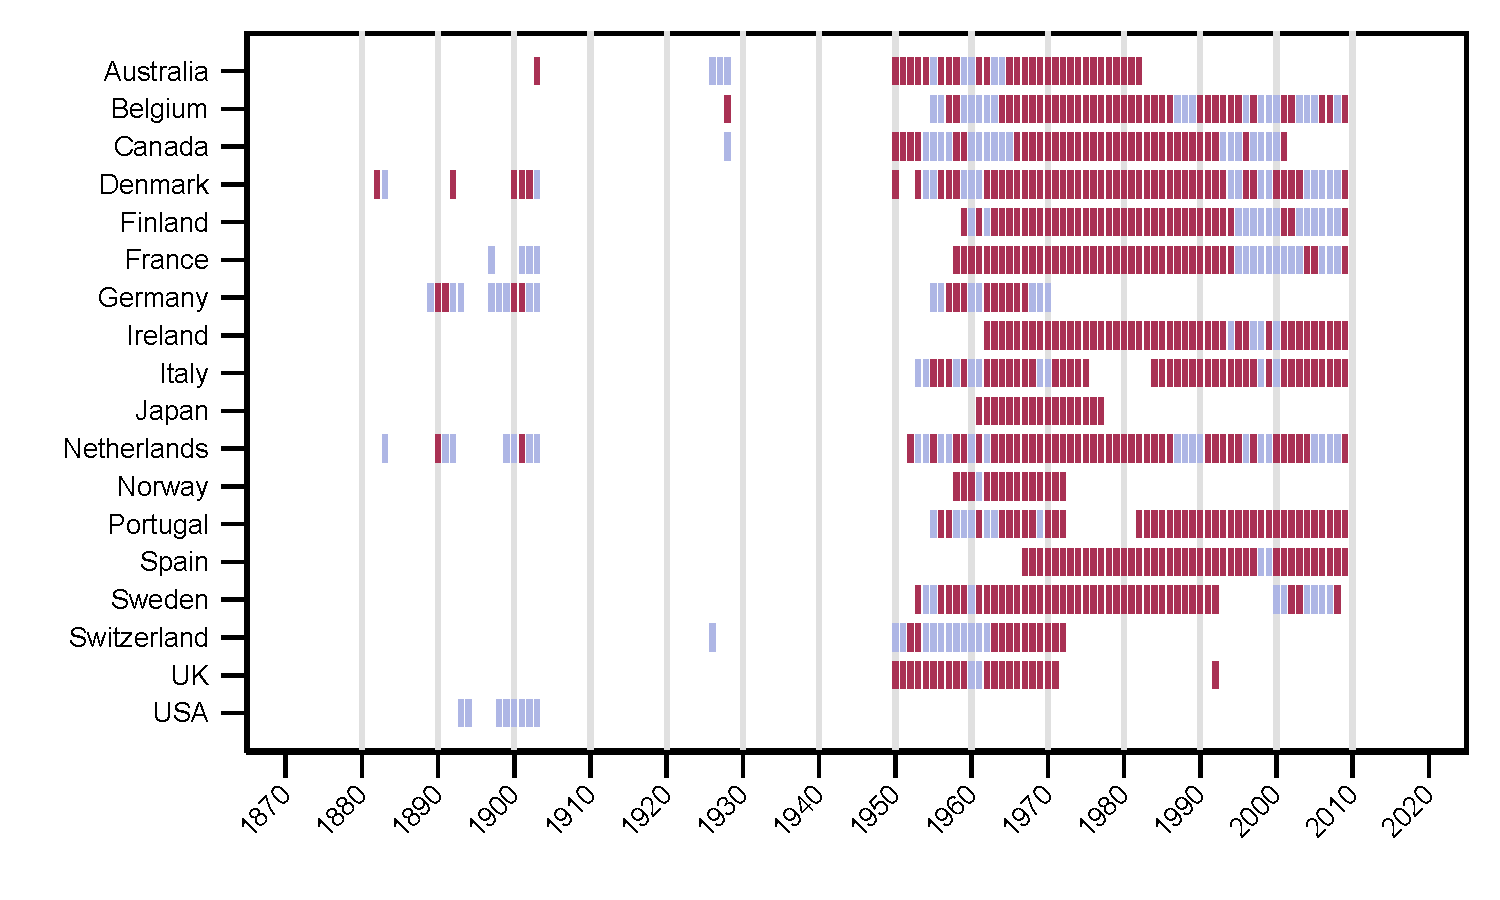
\includegraphics[scale=0.55]{../Output/Figures/history_Sample_SD}
    \annote{\footnotesize This figure displays which year-country observations are being used when estimating the state-dependent Phillips multiplier in periods of high (blue) versus low (red) inflation. Differences to the main sample used (Figure \ref{F:Sample}) represent the periods with inflation smaller than -2\% or above 40\% as per definition.}
    \label{F:Sample_SD}
\end{figure}


\begin{figure}[h!]
    \centering
	\caption{State-Dependent Phillips multiplier and IRFs}
	\label{F:Multiplier_SD_App}
	\begin{subfigure}[b]{0.4\textwidth}
		\caption{Phillips multiplier}
		\label{F2:Multiplier_MM}
		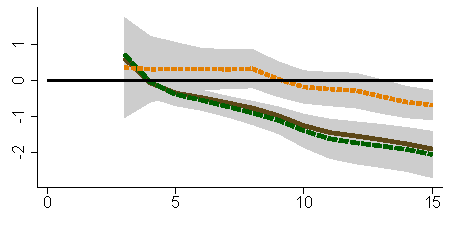
\includegraphics[width=\textwidth]{../Output/Figures/fig_full_SDPMBM_LPIV15_2_asym_lowflat.pdf}	
	\end{subfigure}
	\begin{subfigure}[b]{0.4\textwidth}
		\caption{F-Statistic}
		\label{F2:Multiplier_FF}
		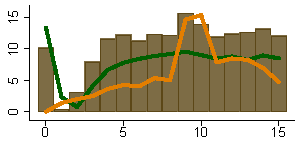
\includegraphics[width=\textwidth]{../Output/Figures/fig_full_PMBM_F_LPIV15_2_asym_lowflat.pdf}
	\end{subfigure}
	\begin{subfigure}[b]{0.8\textwidth}
		\caption{Impulse Responses}
		\label{F2:Dynamics_DD}
		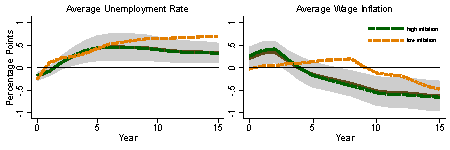
\includegraphics[width=\textwidth]{../Output/Figures/fig_full_SDLPIVBM15_2_asym_lowflat.pdf}
		\end{subfigure}
		\annote{This figure presents a robustness exercise with a higher horizon (15 years) and an unmatched sample, that is, using all available information and abstracting from eventual sample changes across each horizon as the number of observations decreases from 1000 to approximately 650. Here, I also control for two lags of unemployment and wage inflation, country fixed effects, and world GDP growth. The \cite{Olea2013} effective F-statistic of the IRFs are around 30 and 50, for unemployment and wage inflation respectively, and always above the 10\% TSLS threshold. Figures display 90\% confidence bands for the baseline scenario. The state-dependent multipliers are significantly different for horizons between years 9 and 12 as one can confirm in Table \ref{T:SDPM_App}. Across all figures, one can distinguish the state by its color and shape, short-dashed orange shape for low inflation and long-dashed green shape for high inflation.}
	
\end{figure}


\begin{figure}[h!]
    \centering
	\caption{Quarterly Data Phillips multiplier and IRFs}
	\label{F:MultiplierQ}
	\begin{subfigure}[b]{0.45\textwidth}
		\caption{Phillips multiplier}
		\label{F:MultiplierQ_M}
		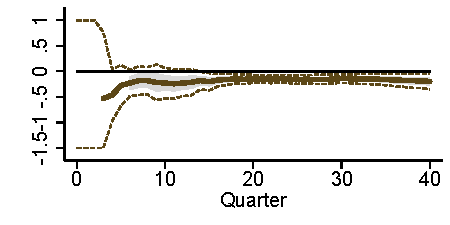
\includegraphics[width=\textwidth]{../Output/Figures/fig_full_PMBM_LPIV40_2_Quarter.pdf}	
	\end{subfigure}
	\begin{subfigure}[b]{0.45\textwidth}
		\caption{F-Statistic}
		\label{F:MultiplierQ_F}
		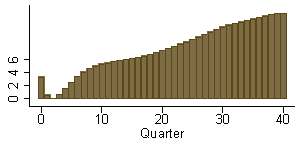
\includegraphics[width=\textwidth]{../Output/Figures/fig_full_PMBM_F_LPIV40_2_Quarter.pdf}
	\end{subfigure}
	\begin{subfigure}[b]{0.9\textwidth}
		\caption{Impulse Responses}
		\label{F:DynamicsQ}
		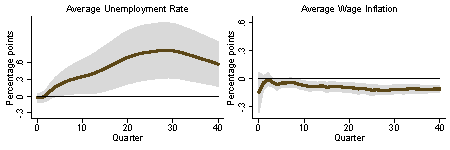
\includegraphics[width=\textwidth]{../Output/Figures/fig_full_LPIVBM40_2_Quarter.pdf}
		\end{subfigure}
		\annote{Phillips multiplier estimations using the trilemma IV as an instrument, using a matched sample of 465 quarterly observations between 1995q1 and 2019q4, and controlling for two lags of unemployment and wage inflation, country fixed effects, and world GDP growth as explained in Equation \eqref{EQ:MULT}. For the multiplier (upper-left), the shaded area corresponds to the 90\% confidence interval implied by the normal limiting distribution of the 2SLS estimator, while the dashed lines correspond to the two-sided 90\% Anderson-Rubin confidence sets robust to weak instruments. The F-statistics (upper-right) are computed using the method presented in \cite{Olea2013}. The impulse responses (bottom panels) for \textit{average} wage inflation and \textit{average} unemployment are obtained from the OLS regressions \eqref{EQ:IRF} and display 90\% confidence sets.}
	
\end{figure}


\begin{figure}[h!]
    \centering
    \caption{Sample composition for state-dependent quarterly Phillips multiplier estimation}
    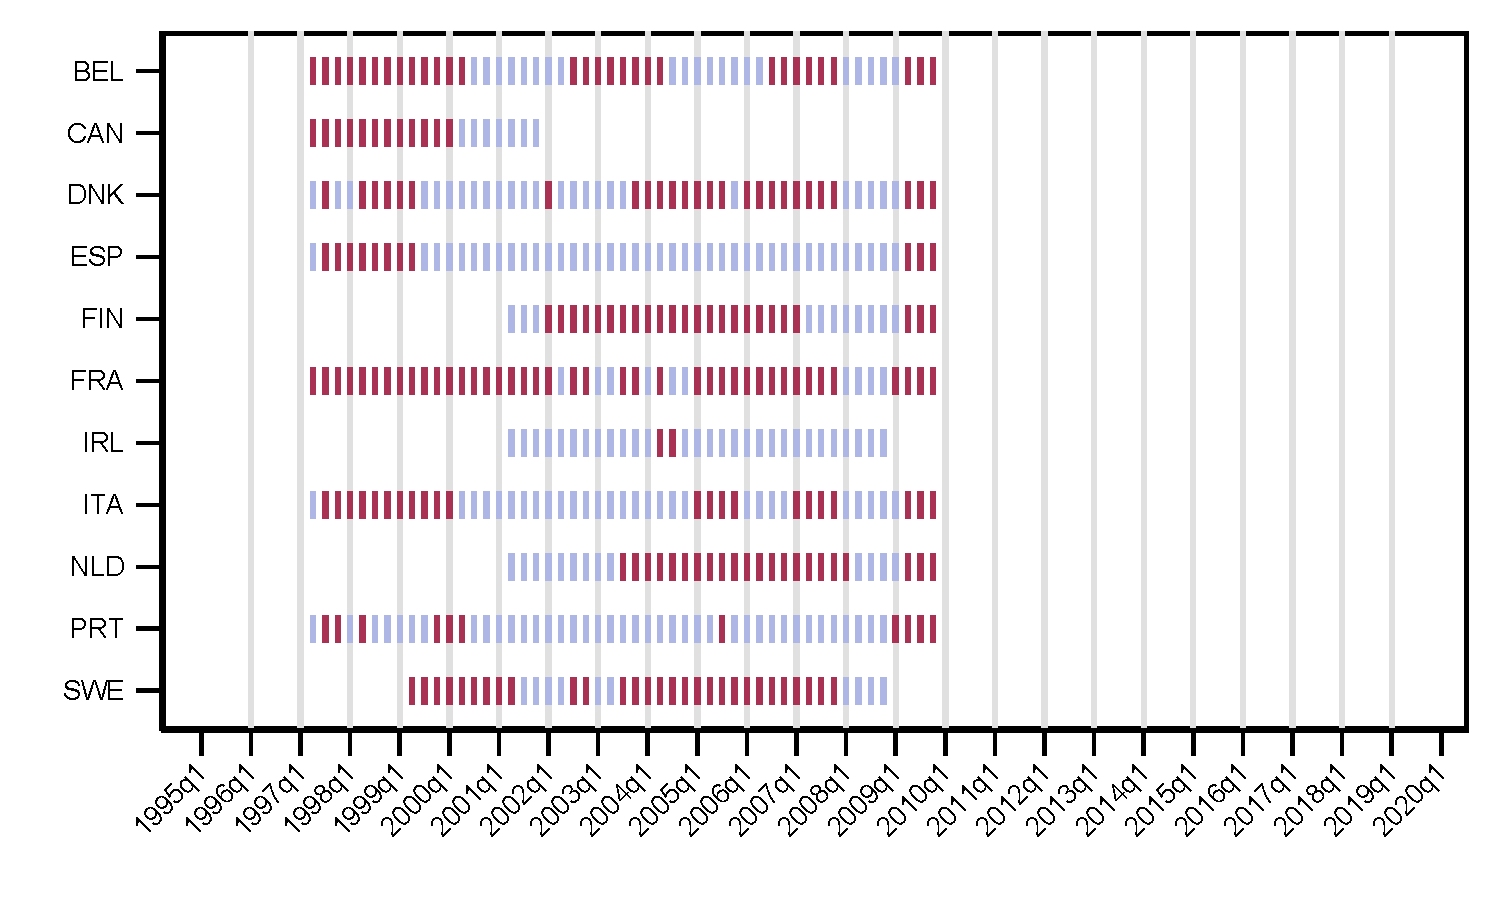
\includegraphics[scale=0.55]{../Output/Figures/history_Sample_SD_quarter}
    \annote{\footnotesize This figure displays which year-country observations are being used when estimating the state-dependent Phillips multiplier in periods of high (blue) versus low (red) inflation.}
    \label{F:SampleQ_SD}
\end{figure}

%\begin{figure}[h]
%    \centering
%	\caption{Policy rate hikes versus cuts - IRFs}
%	\begin{subfigure}[b]{0.9\textwidth}
%		\label{F2:Dynamics_negpos}
%		\includegraphics[width=\textwidth]{../Output/Figures/fig_full_SDLPIVBM10_2_asym_negpos.pdf}
%		\annote{This figure presents the response of cumulative average unemployment and wage inflation for the baseline and another state-dependency on whether there was a policy rate hike (positive first-difference in the variable short-term interest rate) or a policy rate cut (negative change). I control for two lags of unemployment and wage inflation, country fixed effects, and world GDP growth. Figures display 90\% confidence bands for the baseline scenario.}
%	\end{subfigure}
%\end{figure}

\clearpage

\setcounter{table}{0}
\setcounter{figure}{0}

\section{Historical periods} \label{SS_HistoricalPeriods}

It is important to have clearly and coherently identified historical periods as we proceed to a deeper investigation of the research question. Table \ref{T_HistoricalPeriodsSource1} underlies this analysis. It summarizes the allocation of countries to historical periods and their sources. Given that the main channel being analyzed is the low inflation environment, it is crucial to know when countries were targeting either the price of gold or some type of consumer price index.

%In order to make each period comparable to each other, I needed to find a balance between having roughly the same number of observations while guaranteeing that they were historically accurate. 
Identifying the periods of the \textit{Gold Standard}, the \textit{Bretton Woods} and the \textit{Explicit Inflation Targeting} is straightforward. It is based on documented evidence on which countries were participating in one of the above mentioned regimes by either keeping their exchange rate fixed to the price of gold or by targeting inflation.\footnote{One can be wary about whether some countries during the Bretton Woods era were indeed acting accordingly to the agreement (e.g. France as in \cite{Bordo1995}) nonetheless, I am only looking at the participation.}

Dates for the Gold Standard come from \cite{Reinhart2009} and can be confirmed using different sources such as \cite{Bordo1996} and \cite{Diebold1991}. Dates for the Bretton Woods and the Explicit Inflation Targeting come from Central Banks' websites and were complemented by data from \cite{Ilzetzki2019}. Even though the countries present in the Bretton Woods system agreement (1944) started to progressively adopt a fixed exchange rate, I define the start of the Bretton Woods era in 1946 after the creation of the International Monetary Fund (IMF) in December, 1945.\footnote{The starting dates for most countries coincide with the effective date of IMF membership available online \href{https://www.imf.org/external/np/sec/memdir/memdate.htm}{here}. Nevertheless, I acknowledge that if a country had its currency pegged to a major currency such as the US dollar, it is expected that they were implicitly ``part of" the Bretton Woods system.} The Bretton Woods system broke down on 15 August, 1971 thus, I decided to classify 1971 as the last effective year of this epoch.
%One could argue that the system truly became operational in 1958 when the conversion of currency became tied to the U.S. dollar, with the exchange rate around the world based on the figure of \$35 per ounce of gold. Nevertheless, given the focus of my analysis it suffices to do a robustness check here by using the exchange rate peg definition from \cite{Jorda2017}.

The first World War went from July 1914 to November 1918 while the second World War started on September, 1939 and ended on September, 1945. Consequently, it was easy to define the \textit{Interwar Period} with the caveat of choosing 1922 as the beginning of this period to remove the effects of the post-war recession mostly felt in Europe, a common practice in the literature.

%Even though some countries remained neutral in one or even both Wars, the entire sample was significantly affected and thus, I do not consider these periods and their aftermaths in my baseline estimates. Nevertheless, in Section \ref{S_With}, I consider all available observations and the main results go through.

Finally, one needs to argue on the exact year when countries started implicitly targeting inflation. While explicit inflation targeting, in the sense of it being announced by the national Central Banks, started only in the nineties, there is a long literature arguing that some countries were implicitly doing it before that.

According to \cite{vonHagen1999}, ``\textit{the Bundesbank began to announce inflation targets together with adopting monetary targeting, first a series of `unavoidable’ inflation rates and, from 1986 on, a fixed rate of 2\%}".\footnote{Some others would agree on a date even before 1986 \citep{Mishkin2001}.} The German Mark accounted for roughly one-third of the weight of the European Currency Unit (ECU) value from 1984 until 1999. Given both Germany's importance to the ECU and its adoption of an inflation target, I am considering that countries who already belong to the European Exchange Rate Mechanism (EERM) such as Denmark, France, Ireland, Italy, Netherlands and then countries who later join the EERM as Belgium, Finland, Portugal, Spain and the UK or pegged their currencies to the ECU such as Norway and Sweden, are implicitly adopting a behavior of targeting price inflation. For Japan, this definition is based on the work of \cite{Jinushi2000} who thoroughly explains why Japan was implicitly targeting inflation by 1987.

\cite{Ungerer1997}, page 183, tells us that Norway and Sweden pegged their currency to the ECU and in 1990 and 1991 respectively. Even though they abandoned such a peg later on, both of them became explicit inflation targeters - Norway in 2001 and Sweden in 1993. 

UK was a member of the ERM from October 1990 to September 1992. Shortly after, it became the first explicit inflation targeter in Europe. Finally, and even though only in 2012 did the FED announce its explicit target to inflation, \cite{Goodfriend2004} argues that \textit{``monetary policy as conducted in the Greenspan era can be characterized as implicit inflation targeting"}, hence, I consider that in 1988 the USA was an implicit targeter.

According to \cite{Berg1999}, Sweden had an experience similar to inflation targeting between 1931-1937 thus undergoing into an attempt to mimic the price stabilization features of the gold standard while eliminating the volatility produced by shocks to the gold market. 

\begin{landscape}
\begin{table}[]
\caption{Allocation of countries to historical periods} 
\label{T_HistoricalPeriodsSource1}
\centering 
\scriptsize
\def\sym#1{\ifmmode^{#1}\else\(^{#1}\)\fi} 
\begin{longtable}{l*{1}{cccc|c}}
\hline\hline
                    &\multicolumn{1}{c}{\textbf{Gold Standard}}&\multicolumn{1}{c}{\textbf{Bretton Woods}}&\multicolumn{1}{c}{\textbf{Implicit Inflation Target}}&\multicolumn{1}{c}{\textbf{Explicit Inflation Target}}&\multicolumn{1}{c}{\textbf{CB Foundation}}\\
\hline
\textbf{Australia} & 1870-1915 & 1949-1971 & 1993-2020 & 1993-2020 & 1911 \\
           & \cite{Reinhart2009} &\href{https://www.rba.gov.au/speeches/1997/sp-gov-290997.html}{Reserve Bank of Australia} & \href{https://www.rba.gov.au/speeches/1997/sp-gov-290997.html}{Reserve Bank of Australia} & \href{https://www.rba.gov.au/speeches/1997/sp-gov-290997.html}{Reserve Bank of Australia} \\
[1ex]
\textbf{Belgium}  & 1878-1914   & 1946-1971 & 1990-2020 & no & 1850 \\
         & RR \citeyear{Reinhart2009}   & \href{https://www.nbb.be/en/notes-and-coins/belgian-currency/history-belgian-franc/1945-2002-rise-and-disappearance-belgian}{National Bank of Belgium} & \href{https://www.nbb.be/en/notes-and-coins/belgian-currency/history-belgian-franc/1945-2002-rise-and-disappearance-belgian}{National Bank of Belgium} & \\
[1ex]
\textbf{Canada}   & 1870-1914 & 1946-1950 / 1962-1971 & 1991-2020 & 1991-2020 & 1934\\
         & RR \citeyear{Reinhart2009}   & Bordo et al. \citeyear{Bordo2010} & \href{https://www.bankofcanada.ca/wp-content/uploads/2011/12/bocreview-mar1991.pdf}{Bank of Canada} & \href{https://www.bankofcanada.ca/wp-content/uploads/2011/12/bocreview-mar1991.pdf}{Bank of Canada} & \\
[1ex]
\textbf{Denmark}    & 1876-1917 & 1946-1971 & 1986-2018  & no & 1818 \\
    & RR \citeyear{Reinhart2009} & \href{http://www.nationalbanken.dk/EditorImages/Artikel\%20billeder/Danmark\%20Nationalbank\%20200aar_stor_uk.jpg}{Danmarks Nationalbank} & \href{http://www.nationalbanken.dk/EditorImages/Artikel\%20billeder/Danmark\%20Nationalbank\%20200aar_stor_uk.jpg}{Danmarks Nationalbank} & & \\
[1ex]
\textbf{Finland}  & 1877-1914  & 1948-1971  & 1995-2020 & no & 1811 \\
         & RR \citeyear{Reinhart2009} & \href{https://www.suomenpankki.fi/en/bank-of-finland/history/}{Suomen Pankki}  & \href{https://www.suomenpankki.fi/en/bank-of-finland/history/}{Suomen Pankki}  & & \\
[1ex]
\textbf{France}     & 1878-1914  & 1946-1971  & 1986-2020 & no & 1800\\
    & RR \citeyear{Reinhart2009} & \href{https://www.banque-france.fr/en/page-sommaire/history}{Banque de France}  & \href{https://www.banque-france.fr/en/page-sommaire/history}{Banque de France} &  \\
[1ex]
\textbf{Germany} & 1871-1914 & 1952-1971 & 1986-2020 & no & 1876 \\
    & RR \citeyear{Reinhart2009} & \href{https://www.bundesbank.de/de/presse/pressematerial/60-jahre/rechtlicher-rahmen}{Bundesbank}  & \cite{vonHagen1999}   &  \\
[1ex]
\textbf{Italy}  & 1884-1917 & 1947-1971 & 1986-2020 & no & 1893\\
         & RR \citeyear{Reinhart2009}    & \href{https://www.bancaditalia.it/chi-siamo/storia/seconda-guerra-mondiale/index.html}{Banca D'Italia} & \href{https://www.bancaditalia.it/chi-siamo/storia/anni-cinquanta/index.html}{Banca D'Italia} &  \\
[1ex]
\textbf{Japan}  & 1897-1917 & 1952-1971 & 1987-2020 & 2012-2020 & 1882\\
         & RR \citeyear{Reinhart2009} & \cite{Shizume2018} & Jinushi et al. \citeyear{Jinushi2000} & \href{https://www.boj.or.jp/en/announcements/release_2012/k120214b.pdf}{Bank of Japan} & \\
[1ex]
\textbf{Netherlands}  & 1875-1914 & 1946-1971 & 1986-2020 & no & 1814\\
         & RR \citeyear{Reinhart2009} & \href{https://www.dnb.nl/en/about-dnb/organisation/history/index.jsp}{De Nederlandsche Bank} & \href{https://www.dnb.nl/en/about-dnb/organisation/history/index.jsp}{De Nederlandsche Bank} &  & \\
[1ex]
\textbf{Norway}    & 1875-1914 & 1946-1971 & 1990-2020 & 2001-2020 & 1816 \\
    & RR \citeyear{Reinhart2009} & \href{https://www.norges-bank.no/en/topics/about/History/Norges-Banks-history/}{Norges Bank}  & \href{https://www.norges-bank.no/en/topics/about/History/Norges-Banks-history/}{Norges Bank} & \href{https://www.norges-bank.no/en/topics/about/History/Norges-Banks-history/}{Norges Bank} & \\
[1ex]
\textbf{Portugal}  & 1870-1891  & 1961-1971 & 1992-2020 & no & 1846\\
         & RR \citeyear{Reinhart2009}  &  \cite{Bordo1995B}  & \href{https://www.bportugal.pt/}{Banco de Portugal} &  \\
[1ex]
\textbf{Spain}  & |  & 1958-1971 & 1990-2020 & no & 1874\\
         & RR \citeyear{Reinhart2009}  & \href{https://www.bde.es/bde/en/}{Banco de España} & \href{https://www.bde.es/bde/en/}{Banco de España} &  & \\
[1ex]
\textbf{Sweden}    & 1873-1914  & 1951-1971  & 1991-2020 & 1993-2020 & 1668\\
    & RR \citeyear{Reinhart2009}  & \href{https://www.riksbank.se/en-gb/about-the-riksbank/history/}{Sveriges Riksbank} & \href{https://www.riksbank.se/en-gb/about-the-riksbank/history/}{Sveriges Riksbank} & \href{https://www.riksbank.se/en-gb/about-the-riksbank/history/}{Sveriges Riksbank} \\
[1ex]
\textbf{Switzerland}  & 1878-1914  & 1946-1971 & 1986-2020 & no & 1907 \\
         & RR \citeyear{Reinhart2009}  & \cite{Baltensperger2017} &  \href{https://www.snb.ch/en/iabout/snb/hist/id/hist_wpc}{Swiss National Bank} &  & \\
[1ex]
\textbf{UK}       & 1870-1914 & 1946-1971  & 1991-2020 & 1992-2020 & 1694\\
    & RR \citeyear{Reinhart2009} & \cite{Bordo1999}  & \href{https://www.bankofengland.co.uk/about/history}{Bank of England} & \href{https://www.bankofengland.co.uk/about/history}{Bank of England} \\
[1ex]
\textbf{USA}     & 1880-1917 & 1946-1971  & 1988-2020  & 2012-2020  & 1913\\
    & RR \citeyear{Reinhart2009}  & \cite{Bordo1999} & \cite{Goodfriend2004} & FED \\
\hline\hline
\end{longtable}
\vspace{-3ex}
\annote{This Table presents the allocation of countries to historical periods. Further discussion on this follows. All Central Bank Foundations dates were collected from the Central Banks' websites.}
\end{table}
\end{landscape}

%The focus on the explicit targeters in the main analysis was based on the objectivity of the measure - it is straightforward to associate the start of the inflation targeting period to one communication from the respective central bank. Nevertheless, the case for implicit inflation targeting is also analyzed in appendix \ref{S_ImplicitIT} and the results of this paper hold for both definitions.

%Mostly via the rolling-window regressions, I study the wage Phillips curve in each of these periods. As commonly done in the literature, I am explicitly excluding some of the arguably dark periods of the world wars (1914-1919 and 1939-1945, excluding the USA which only entered the first world war in April 1917), the hyperinflation in Germany (1920-1926), and the Great Depression in the USA (1929-1941)  \cite{Bordo2018}.\footnote{In appendix \ref{S_With}, I replicate the results with all the available data and the results qualitatively hold.}




\clearpage

\setcounter{table}{0}
\setcounter{figure}{0}
\setcounter{Equation}{0}

\section{The New Keynesian wage Phillips curve: a panel framework \label{S_Theory}}

In this Appendix section, I derive a panel version of the New Keynesian wage Phillips curve following closely the work from \cite{Gali2011} and \cite{Erceg2000} on staggered wage contracts. Then, I explore the mechanisms which might lead to changes in the Phillips curve slope across time.

As in \cite{Gali2011}, the variant of the staggered wage setting model from \cite{Erceg2000} presented here assumes that labor is indivisible. Furthermore, I assume that there are $C$ countries, indexed by $c$, in order to add a panel component.

In each country, there is a (large) representative household with a continuum of members represented by the unit square and indexed by a pair $(i,j) \in [0,1] \times [0,1]$. Where the first dimension represents the type of labor service in which a given household member is specialized and the second one determines the member's disutility from work. The latter is given by:
\[ 
\left\{
\begin{array}{ll}
      \chi_{c,t} \ j^{\phi} & if \ employed \\
      0 & if \ unemployed
\end{array} 
\right. 
\]
where $\phi \geq 0$ determines the elasticity of the marginal disutility of work and $\chi_{c,t} > 0$ is a country-specific and exogenous labor supply shock which may shift the marginal rate of substitution between consumption and leisure over time.

The utility is logarithmic in consumption and there is full risk sharing among household members. The household period utility is described as:

    \begin{Equation*}
        U(C_{c,t},\{N_{c,t}(i)\}, \chi_{c,t}) \equiv log(C_{c,t}) - \chi_{c,t} \int_0^1 \int_0^{N_{c,t}(i)} j^{\phi} dj di
    \end{Equation*}
    \begin{Equation*}
        \indent \indent \indent \indent \indent  = log(C_{c,t}) - \chi_{c,t} \int_0^1 \dfrac{N_{c,t}(i)^{1+\phi}}{1+\phi} di
    \end{Equation*}
where $C_{c,t}$ denotes the household consumption, and $N_{c,t}(i) \in [0,1]$ is the fraction of members specialized in type $i$ labor who are employed in period $t$ in country $c$. In each country, the representative household maximizes:

\begin{Equation*}
    E_0 \sum_{t=0}^{\infty} \beta^t U(C_{c,t},\{N_{c,t}(i)\}, \chi_{c,t})
\end{Equation*}
subject to a sequence of budget constraints
\begin{Equation*}
    P_{c,t} C_{c,t} + Q_{c,t} B_{c,t} \leq B_{c,t-1} + \int_0^1 W_{c,t}(i) N_{c,t}(i) di + \Pi_t
\end{Equation*}
where $P_{c,t}$ is the price of the consumption bundle. $W_{c,t}(i)$ is the nominal wage for labor of type $i$, $B_{c,t}$ represents purchases of a nominally risk-free one-period bond (at the national price $Q_{c,t}$), and $\Pi_{c,t}$ is a lump-sum component of income.\footnote{As in \cite{Gali2011} the sequence of period budget constraints is supplemented with a solvency condition which prevents the household from engaging in Ponzi schemes.}

% I also assumed a no-arbitrage condition such that, in equilibrium, $P_{c,t} = P_t$ and that $Q_{c,t} = Q_t$ for all $c=1,...,C$.

As in \cite{Erceg2000} and following the formalism of \cite{Calvo1983}, workers supplying a labor service of a given type get to reset their (nominal) wage with probability $(1-\theta)$ each period. For now, I assume that this probability is constant over time and across countries just like the two other parameters $\beta$ and $\phi$. In the next section, I delve further into this issue.

Once the wage has been set, the quantity of workers employed is determined unilaterally by firms, with households willingly meeting that demand (given that the wage remains above the disutility of work for the marginal worker). When workers reoptimize their wage in period t, they do so by choosing a wage $W_{c,t}^*$ such that the following first order condition holds:\footnote{For details of the optimal wage setting condition derivation see \cite{Erceg2000}.}

\begin{Equation*}
    \sum_{k=0}^{\infty} (\beta \theta)^k E_t \Bigg[ \frac{N_{c,t+k|t}}{C_{c,t+k}} \Bigg( \dfrac{W_t^{c*}}{P_{c,t+k}} - \mathcal{M}_c MRS_{c,t+k|t} \Bigg) \Bigg] = 0
\end{Equation*}
where $N_{c,t+k|t}$ denotes the quantity demanded in period $t+k$ of a labor type whose wage is being reset in period $t$, $MRS_{c,t+k|t} \equiv \chi_{c,t+k} C_{c,t+k} (N_{c,t+k|t})^\phi$ is the relevant marginal rate of substitution between consumption and employment in period $t+k$, and $\mathcal{M}_c \equiv \dfrac{\epsilon_c}{(\epsilon_c - 1)}$ is the desired (or flexible wage) markup, with $\epsilon_c$ denoting the wage elasticity of demand for the services of each labor type assumed to be constant over time.\footnote{See \cite{Gali2012} for an application of a one-country framework allowing for time variations in the desired wage markup.}

Log-linearizing the above optimality condition around a perfect foresight zero inflation steady state, using lower case letters to denote the logs of the corresponding variable and letting $\mu_c \equiv log(\mathcal{M}_c)$, we obtain the approximate wage setting rule:
\begin{Equation}
    w_{c,t}^{*} = \mu_c + (1-\beta \theta) \sum_{k=0}^{\infty} (\beta \theta)^k E_t [mrs_{c,t+k|t}+p_{c,t+k}] 
\end{Equation}

When nominal wage rigidities are present $(\theta > 0)$, new wages are set as a constant markup over a weighted average of current and expected future price-adjusted marginal rates of substitution. Furthermore, log-linearizing the expression for the aggregate wage index around a zero inflation steady state we obtain:
\begin{Equation}
    w_{c,t} = (1-\theta)w_{c,t}^* + \theta w_{c,t-1}
\end{Equation}
Moreover, letting $mrs_{c,t} \equiv c_{c,t} + \phi n_{c,t} + \xi_{c,t}$ denote the economy’s average (log) marginal rate of substitution, with $\xi_{c,t} = log(\chi_{c,t})$, we can write:
\begin{Equation}
    mrs_{c,t+k|t} = mrs_{c,t+k} - \epsilon_c \phi (w_{c,t}^* - w_{c,t+k})
\end{Equation}
I proceed to combine Equations (1) through (3) in order to derive the baseline wage Equation in each country $c$:
\begin{Equation}
    \label{EQ_baseline}
    \pi_{c,t}^{w} = \beta E_t [\pi_{c,t+1}^{w}] + \lambda_c (\mu_{c,t} - \mu_c)
\end{Equation}
where $\pi_{c,t}^{w} \equiv w_{c,t} - w_{c,t-1}$ is wage inflation, $\mu_{c,t} \equiv w_{c,t} - p_{c,t} - mrs_{c,t}$ denotes the (average) wage markup in country $c$ and $\mu_{c,t} - \mu_c$ is the natural wage markup, the gap between the average real wage and the marginal rate of substitution that would prevail under flexible prices. By assumption, we then have $\lambda_c \equiv - \dfrac{(1-\theta)(1-\beta \theta)}{\theta (1+\epsilon_c \phi)} < 0$. 

Even though this relation holds irrespective of the wage setting process, I further assume partial indexation of wages to a measure of lagged price inflation ($\pi^p_{t-1}$) when there is no reoptimization of wages, with probability $\theta$ each period. Such assumption is reasonable when we consider that there exists a strong positive correlation between wage inflation ($\pi_t^w$) and lagged price inflation ($\pi^p_{t-1}$) at the country level as showed in Table \ref{T_Correlation}. Following \cite{Gali2019}, this changes Equation (\ref{EQ_baseline}) to:

\begin{Equation*}
    \tilde{\pi}_{c,t}^{w} = \beta E_t [\tilde{\pi}_{c,t+1}^{w}] + \lambda_c (\mu_{c,t} - \mu_c)
\end{Equation*}

where $\tilde{\pi}_{c,t}^{w} \equiv \pi^w_{c,t} - [\gamma \pi^p_{t-1} + (1-\gamma)\pi]$ and $\gamma$ is the degree of indexation. Further assuming that the natural wage markup follows an AR(1) with persistence $\rho^w$ one can re-write the previous Equation as:

\begin{Equation}
    \label{EQ_baseline2}
    \tilde{\pi}_{c,t}^{w} = \dfrac{\lambda_c}{1 - \beta \rho^w}  (\mu_{c,t} - \mu_c)
\end{Equation}

Next, I introduce unemployment explicitly in the model. Following \cite{Gali2011}, an household member $(i,j)$ uses a household welfare criterion to decide whether she finds it optimal to participate in the labor market. She does so whenever the real wage prevailing in her trade is above her disutility from working, that is, if and only if:
\begin{Equation*}
    \dfrac{W_{c,t}(i)}{P_{c,t}} \geq \chi_{c,t} C_{c,t} j^{\phi}
\end{Equation*}
Thus, the marginal supplier of type $i$ labor (employed or unemployed) in country $c$, which I denote by $L_{c,t}(i)$, is implicitly given by:
\begin{Equation*}
    \dfrac{W_{c,t}(i)}{P_{c,t}} = \chi_{c,t} C_{c,t} L_{c,t}(i)^{\phi}
\end{Equation*}
Log-linearizing and aggregating yields:
\begin{Equation}
    \label{EQ_5}
    w_{c,t} - p_{c,t} = c_{c,t} + \phi l_{c,t} + \xi_{c,t}
\end{Equation}
where $l_{c,t} \equiv \int_0^1 l_{c,t}(i) di$ can be interpreted as the model’s implied labor force, and $w_{c,t} \equiv \int_0^1 w_{c,t}(i) di$ is the average wage, both expressed in logs. Naturally, the unemployment rate can be defined as:
\begin{Equation}
    \label{EQ_6}
    u_{c,t} \equiv l_{c,t} - n_{c,t}
\end{Equation}
Combining Equations (\ref{EQ_5}) and (\ref{EQ_6}) with the expression for the average wage markup $\mu_{c,t}$ yields the following linear relation between the wage markup and the unemployment rate:
\begin{Equation}
    \label{EQ_u}
    u_{c,t} = \mu_{c,t} \phi^{-1} 
\end{Equation}
Let us define the natural rate of unemployment, $u_{c,t}^n$, as the rate of unemployment that would prevail in the absence of nominal wage rigidities. It follows from the assumption of a constant desired wage markup that $u_{c,t}^n$ is constant and given by:
\begin{Equation}
    \label{EQ_un}
    u_{c}^n = \mu_c \phi^{-1}
\end{Equation}
Thus, in the framework above unemployment is a consequence of workers’ market power (that is, of the wage being above their perfectly competitive level), while unemployment fluctuations result from the slow adjustment of wages. 
%Figure \ref{F_Gali_2011} represents the relation between the wage markup and the unemployment rate using a simple diagram of the labor market.

Finally, combining Equations (\ref{EQ_baseline2}), (\ref{EQ_u}) and (\ref{EQ_un}) and defining $\varphi_c \equiv \dfrac{\phi \lambda_c}{1 - \beta \rho^w}$ we obtain the following panel version of a New Keynesian wage Phillips curve (henceforth, NKWPC):
\begin{Equation}
    \label{EQ_NKWPC}
    \pi_{c,t}^{w} = (1-\gamma)\pi + \gamma \pi^p_{t-1} + \varphi_c (u_{c,t} - u_c^n)
\end{Equation}

\subsection{A time-varying New Keynesian wage Phillips curve \label{SS_FPA}}

A classical assumption across existing studies on the Phillips curve is to have time-invariant parameters $(\beta, \theta, \epsilon, \phi)$. Notwithstanding, one should be wary of it when estimating a Phillips curve using such long samples as this current work. An economy arguably changes within 150 years. 

\cite{Romer1990} argued that the frequency of price (wage) adjustments was likely to vary in response to the volatility of the economic environment. In particular, he claimed that the frequency would be lower in an environment of low inflation with lower volatility. This belief is corroborated by the recent empirical works of \cite{Gagnon2009} and \cite{Nakamura2018}. 

Some literature followed this assumption either by modeling time-varying parameters as random variables \citep{Romer1990, Primiceri2005} or by allowing for different parameters in different sub-sample periods \citep{Gali1999, Smets2007}.

In this work, given its historical perspective, I assumed that the model parameters might vary across time and make use of a rolling window estimation to motivate the main finding of the paper. From Equation \eqref{EQ_NKWPC}, one can see how the slope responds to the parameters by looking at its definition:
\begin{Equation*}
    \varphi \equiv - \dfrac{\phi (1-\theta)(1-\beta \theta)}{(1 - \beta \rho^w) \theta (1+\epsilon \phi)} < 0   
\end{Equation*}

\begin{figure}[ht!]
	\centering
	\caption{Slope of the NKWPC \label{F:NKWPCslope}}
	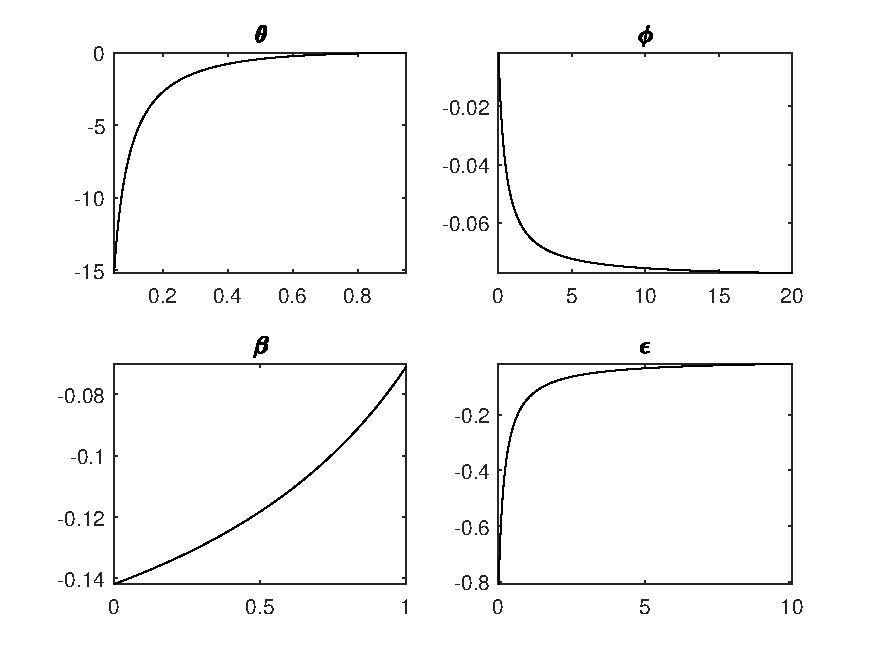
\includegraphics[width=0.7\textwidth]{../Output/Figures/NKWPCslope.pdf} 
	\annote{\footnotesize Calibration. The discount factor, $\beta$ is set to 0.99 and the persistence of the natural wage markup gap $\rho^w$ is set to 0.5. The Calvo wage stickiness parameter, $\theta$, imply an average duration of individual wages of one year, in a way consistent with much of the micro evidence \cite{Nakamura2008}. The curvature of labor disutility, $\phi$, is set to be 5, a value consistent with a Frisch labor elasticity of 0.2. \cite{Gali2011} shows that $\phi$, $\epsilon$, and the steady-state unemployment rate $u$ have the following relationship: $\phi u = log(\epsilon / (\epsilon -1))$. Given that $\phi$ is set to 5, the value of $\epsilon$ is set to 2.15. This is consistent with a steady-state unemployment rate of 5.4 percent, the average unemployment rate in the full sample (Table \ref{T:Descriptives}). }
\end{figure}


The slope of the NKWPC is negative by assumption. The relation between the slope and the remaining parameters can be found in Figure \ref{F:NKWPCslope}. Given the support of its fundamental parameters, it depends positively and strongly on $\theta$. 

If firms adjust prices more frequently, the NKWPC slope decreases in absolute value. Therefore, one expects that in periods of lower inflation, firms adjust prices and wages less often thus flattening the slope of the Phillips curve \citep{Benati2007}. This rationale is in line with two strands of the literature.\footnote{It is not the focus of this paper to test which theory is more suitable but rather test whether in periods of low inflation we see a weaker wage inflation-unemployment tradeoff.}

The theoretical state dependent pricing literature states that, at low inflation levels, the frequency of wage (price) adjustment decreases. Since workers and firms respond less to shocks at low inflation, the overall price level also becomes less reactive, leading to a substantially flatter Phillips curve \citep{Costain2022}.

An alternative argument hinges on the theory of nominal price rigidities (\cite{Tobin1972}, \cite{Akerlof1996}, \cite{Benigno2011}, \cite{Daly2014}, \cite{Gagnon2019}, \cite{Linde2019}). It claims that during periods of low inflation, nominal wages (prices) tend to be more rigid downwards than upwards and thus, they will react less to changes in the unemployment rate.



\clearpage


\begin{comment}

\setcounter{table}{0}
\setcounter{figure}{0}

\section{Historical periods} \label{SS_HistoricalPeriods}

It is important to have clearly and coherently identified historical periods as we proceed to a deeper investigation of the research question. Table \ref{T_HistoricalPeriodsSource1} underlies this analysis. It summarizes the allocation of countries to historical periods and their sources. Since the main channel being analyzed is the low inflation environment, it is crucial to know when countries were targeting either the price of gold or some type of consumer price index.

%In order to make each period comparable to each other, I needed to find a balance between having roughly the same number of observations while guaranteeing that they were historically accurate. 
Identifying the periods of the \textit{Gold Standard}, the \textit{Bretton Woods} and the \textit{explicit inflation targeting} is straightforward. It is based on documented evidence on which countries were participating in one of the above-mentioned regimes by either keeping their exchange rate fixed to the price of gold or targeting inflation.\footnote{One can be wary about whether during the Bretton Woods era some countries were acting according to the agreement (e.g. France as in \cite{Bordo1995}) nonetheless, I am only looking at the participation.}

The dates of the Gold Standard are from the study of \cite{Reinhart2009} and can be confirmed using different sources such as \cite{Bordo1996} and \cite{Diebold1991}. The dates of the Bretton Woods and explicit inflation targeting are from central banks' websites and complemented by data from \cite{Ilzetzki2019}. Although the countries present in the Bretton Woods system agreement (1944) started to progressively adopt a fixed exchange rate, I define the start of the Bretton Woods era from 1946 after the creation of the International Monetary Fund (IMF) in December 1945.\footnote{The starting dates for most countries coincide with the effective date of IMF membership available online \href{https://www.imf.org/external/np/sec/memdir/memdate.htm}{here}. However, I acknowledge that if a country had its currency pegged to a major currency such as the US dollar, it is expected that they were implicitly ``part of" the Bretton Woods system.} The Bretton Woods system broke down on August 15, 1971, so I decided to classify 1971 as the last effective year of this epoch.
%One could argue that the system truly became operational in 1958 when the conversion of currency became tied to the U.S. dollar, with the exchange rate around the world based on the figure of \$35 per ounce of gold. Nevertheless, given the focus of my analysis it suffices to do a robustness check here by using the exchange rate peg definition from \cite{Jorda2017}.

%The first World War lasted from July 1914 to November 1918, whereas the second World War was from September 1939 to September 1945. %Consequently, it was easy to define the \textit{interwar period} with the caveat of choosing 1922 as the beginning of this period to remove the effects of the post-war recession mostly felt in Europe, a common practice in the literature.

%Even though some countries remained neutral in one or even both Wars, the entire sample was significantly affected and thus, I do not consider these periods and their aftermaths in my baseline estimates. Nevertheless, in Section \ref{S_With}, I consider all available observations and the main results go through.

Finally, one needs to argue on the exact year when countries started implicitly targeting inflation. Although explicit inflation targeting, as announced by the national central banks, started only in the nineties, many studies argue that some countries were implicitly doing it before that.

According to \cite{vonHagen1999}, ``\textit{the Bundesbank began to announce inflation targets together with adopting monetary targeting, first a series of `unavoidable' inflation rates and, from 1986 on, a fixed rate of 2\%}".\footnote{Others would agree on a date even before 1986 \cite{Mishkin2001}.} The German Mark accounted for approximately one-third of the weight of the European Currency Unit (ECU) value from 1984 to 1999. Due to Germany's importance to ECU and its adoption of an inflation target, I assume that countries who already belong to the European Exchange Rate Mechanism (EERM), such as Denmark, France, Italy, and the Netherlands, and countries that later joined the EERM, such as Belgium, Finland, Portugal, Spain, and the UK, or pegged their currencies to the ECU, such as Norway and Sweden, are implicitly adopting a behavior of targeting price inflation. For Japan, this definition is based on the work of \cite{Jinushi2000} who thoroughly explained why Japan was implicitly targeting inflation by 1987.

Norway and Sweden pegged their currency to the ECU in 1990 and 1991, respectively. Although they abandoned such peg later on, both of them became explicit inflation targeters — Norway in 2001 and Sweden in 1993. The UK was a member of the ERM from October 1990 to September 1992. Shortly after, it became the first explicit inflation targeter in Europe. Finally, although it was only in 2012 that the FED announced its explicit target to inflation, \cite{Goodfriend2004} argues that \textit{``monetary policy as conducted in the Greenspan era can be characterized as implicit inflation targeting"}, so I assume that starting in 1988 the USA was an implicit targeter.

%According to \cite{Berg1999}, Sweden had experienced similar inflation targeting from 1931 to 1937, thereby attempting to mimic the price stabilization features of the gold standard while eliminating the volatility produced by shocks to the gold market.

\begin{landscape}
\begin{table}[]
\caption{Allocation of countries to historical periods} 
\label{T_HistoricalPeriodsSource1}
\centering 
\scriptsize
\def\sym#1{\ifmmode^{#1}\else\(^{#1}\)\fi} 
\begin{longtable}{l*{1}{cccc|c}}
\hline\hline
                    &\multicolumn{1}{c}{\textbf{Gold Standard}}&\multicolumn{1}{c}{\textbf{Bretton Woods}}&\multicolumn{1}{c}{\textbf{Implicit Inflation Target}}&\multicolumn{1}{c}{\textbf{Explicit Inflation Target}}&\multicolumn{1}{c}{\textbf{CB Foundation}}\\
\hline
\textbf{Australia} & 1870-1915 & 1949-1971 & 1993-2020 & 1993-2020 & 1911 \\
           & \cite{Reinhart2009} &\href{https://www.rba.gov.au/speeches/1997/sp-gov-290997.html}{Reserve Bank of Australia} & \href{https://www.rba.gov.au/speeches/1997/sp-gov-290997.html}{Reserve Bank of Australia} & \href{https://www.rba.gov.au/speeches/1997/sp-gov-290997.html}{Reserve Bank of Australia} \\
[1ex]
\textbf{Belgium}  & 1878-1914   & 1946-1971 & 1990-2020 & no & 1850 \\
         & RR \citeyear{Reinhart2009}   & \href{https://www.nbb.be/en/notes-and-coins/belgian-currency/history-belgian-franc/1945-2002-rise-and-disappearance-belgian}{National Bank of Belgium} & \href{https://www.nbb.be/en/notes-and-coins/belgian-currency/history-belgian-franc/1945-2002-rise-and-disappearance-belgian}{National Bank of Belgium} & \\
[1ex]
\textbf{Canada}   & 1870-1914 & 1946-1950 / 1962-1971 & 1991-2020 & 1991-2020 & 1934\\
         & RR \citeyear{Reinhart2009}   & Bordo et al. \citeyear{Bordo2010} & \href{https://www.bankofcanada.ca/wp-content/uploads/2011/12/bocreview-mar1991.pdf}{Bank of Canada} & \href{https://www.bankofcanada.ca/wp-content/uploads/2011/12/bocreview-mar1991.pdf}{Bank of Canada} & \\
[1ex]
\textbf{Denmark}    & 1876-1917 & 1946-1971 & 1986-2018  & no & 1818 \\
    & RR \citeyear{Reinhart2009} & \href{http://www.nationalbanken.dk/EditorImages/Artikel\%20billeder/Danmark\%20Nationalbank\%20200aar_stor_uk.jpg}{Danmarks Nationalbank} & \href{http://www.nationalbanken.dk/EditorImages/Artikel\%20billeder/Danmark\%20Nationalbank\%20200aar_stor_uk.jpg}{Danmarks Nationalbank} & & \\
[1ex]
\textbf{Finland}  & 1877-1914  & 1948-1971  & 1995-2020 & no & 1811 \\
         & RR \citeyear{Reinhart2009} & \href{https://www.suomenpankki.fi/en/bank-of-finland/history/}{Suomen Pankki}  & \href{https://www.suomenpankki.fi/en/bank-of-finland/history/}{Suomen Pankki}  & & \\
[1ex]
\textbf{France}     & 1878-1914  & 1946-1971  & 1986-2020 & no & 1800\\
    & RR \citeyear{Reinhart2009} & \href{https://www.banque-france.fr/en/page-sommaire/history}{Banque de France}  & \href{https://www.banque-france.fr/en/page-sommaire/history}{Banque de France} &  \\
[1ex]
\textbf{Germany} & 1871-1914 & 1952-1971 & 1986-2020 & no & 1876 \\
    & RR \citeyear{Reinhart2009} & \href{https://www.bundesbank.de/de/presse/pressematerial/60-jahre/rechtlicher-rahmen}{Bundesbank}  & \cite{vonHagen1999}   &  \\
[1ex]
\textbf{Italy}  & 1884-1917 & 1947-1971 & 1986-2020 & no & 1893\\
         & RR \citeyear{Reinhart2009}    & \href{https://www.bancaditalia.it/chi-siamo/storia/seconda-guerra-mondiale/index.html}{Banca D'Italia} & \href{https://www.bancaditalia.it/chi-siamo/storia/anni-cinquanta/index.html}{Banca D'Italia} &  \\
[1ex]
\textbf{Japan}  & 1897-1917 & 1952-1971 & 1987-2020 & 2012-2020 & 1882\\
         & RR \citeyear{Reinhart2009} & \cite{Shizume2018} & Jinushi et al. \citeyear{Jinushi2000} & \href{https://www.boj.or.jp/en/announcements/release_2012/k120214b.pdf}{Bank of Japan} & \\
[1ex]
\textbf{Netherlands}  & 1875-1914 & 1946-1971 & 1986-2020 & no & 1814\\
         & RR \citeyear{Reinhart2009} & \href{https://www.dnb.nl/en/about-dnb/organisation/history/index.jsp}{De Nederlandsche Bank} & \href{https://www.dnb.nl/en/about-dnb/organisation/history/index.jsp}{De Nederlandsche Bank} &  & \\
[1ex]
\textbf{Norway}    & 1875-1914 & 1946-1971 & 1990-2020 & 2001-2020 & 1816 \\
    & RR \citeyear{Reinhart2009} & \href{https://www.norges-bank.no/en/topics/about/History/Norges-Banks-history/}{Norges Bank}  & \href{https://www.norges-bank.no/en/topics/about/History/Norges-Banks-history/}{Norges Bank} & \href{https://www.norges-bank.no/en/topics/about/History/Norges-Banks-history/}{Norges Bank} & \\
[1ex]
\textbf{Portugal}  & 1870-1891  & 1961-1971 & 1992-2020 & no & 1846\\
         & RR \citeyear{Reinhart2009}  &  \cite{Bordo1995B}  & \href{https://www.bportugal.pt/}{Banco de Portugal} &  \\
[1ex]
\textbf{Spain}  & |  & 1958-1971 & 1990-2020 & no & 1874\\
         & RR \citeyear{Reinhart2009}  & \href{https://www.bde.es/bde/en/}{Banco de España} & \href{https://www.bde.es/bde/en/}{Banco de España} &  & \\
[1ex]
\textbf{Sweden}    & 1873-1914  & 1951-1971  & 1991-2020 & 1993-2020 & 1668\\
    & RR \citeyear{Reinhart2009}  & \href{https://www.riksbank.se/en-gb/about-the-riksbank/history/}{Sveriges Riksbank} & \href{https://www.riksbank.se/en-gb/about-the-riksbank/history/}{Sveriges Riksbank} & \href{https://www.riksbank.se/en-gb/about-the-riksbank/history/}{Sveriges Riksbank} \\
[1ex]
\textbf{Switzerland}  & 1878-1914  & 1946-1971 & 1986-2020 & no & 1907 \\
         & RR \citeyear{Reinhart2009}  & \cite{Baltensperger2017} &  \href{https://www.snb.ch/en/iabout/snb/hist/id/hist_wpc}{Swiss National Bank} &  & \\
[1ex]
\textbf{UK}       & 1870-1914 & 1946-1971  & 1991-2020 & 1992-2020 & 1694\\
    & RR \citeyear{Reinhart2009} & \cite{Bordo1999}  & \href{https://www.bankofengland.co.uk/about/history}{Bank of England} & \href{https://www.bankofengland.co.uk/about/history}{Bank of England} \\
[1ex]
\textbf{USA}     & 1880-1917 & 1946-1971  & 1988-2020  & 2012-2020  & 1913\\
    & RR \citeyear{Reinhart2009}  & \cite{Bordo1999} & \cite{Goodfriend2004} & FED \\
\hline\hline
\end{longtable}
\vspace{-3ex}
\annote{This Table presents the allocation of countries to historical periods. Further discussion on this follows. All Central Bank Foundations dates were collected from the Central Banks' websites.}
\end{table}
\end{landscape}



Gold Standard Exercise 

\subsubsection{The Phillips multiplier is smaller during the Gold Standard and the last 20 years}

Motivated by Figure \ref{F:RWIV}, I now test in a more robust empirical setting whether the wage inflation-unemployment tradeoff is different across sub-samples. To be precise, I am going to aggregate the years where inflation was more credibly anchored - the last 20 years (2000-2019) and the Gold Standard epoch (1870-1913) - and compare them against the post-war period (1946-1999) leaving the between-war period (1920-1938) out of this analysis.

Therefore, I estimate Equation \ref{EQ:MULT_State} where $\mathcal{I}_{c,t}$ is an indicator of the post-war period defined as a dummy variable, which is equal to 1 for the years between 1946 and 1999 and equal to 0 for the years where inflation was more credibly anchored. This exercise allows comparing the evolution of the Phillips multiplier in these sub-samples and directly test whether $\mathcal{P}_h^{(\mathcal{I})} = \mathcal{P}_h^{(1-\mathcal{I})}$.

Figure \ref{F2:Multiplier_GS} displays the estimates of both the baseline and state-dependent Phillips multipliers over a 10-year horizon (Figure \ref{F2:Multiplier_M_GS}), their F-statistics (Figure \ref{F2:Multiplier_F_GS}), and their underlying impulse responses (Figure \ref{F2:Dynamics_GS}) in the historical sub-samples.

\begin{figure}[h!]
    \centering
	\caption{State-Dependent Phillips multiplier and IRFs}
	\label{F2:Multiplier_GS}
	\begin{subfigure}[b]{0.45\textwidth}
		\caption{Phillips multiplier}
		\label{F2:Multiplier_M_GS}
		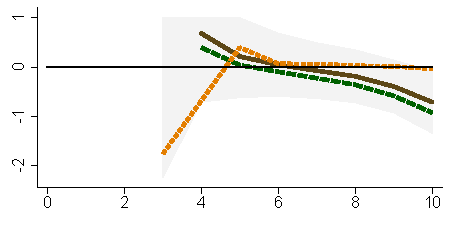
\includegraphics[width=\textwidth]{../Output/Figures/fig_full_SDPMBM_LPIV10_2_asym_postwar.pdf}	
	\end{subfigure}
	\begin{subfigure}[b]{0.45\textwidth}
		\caption{F-Statistic}
		\label{F2:Multiplier_F_GS}
		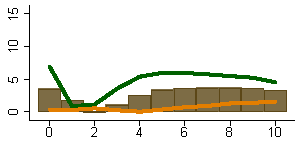
\includegraphics[width=\textwidth]{../Output/Figures/fig_full_PMBM_F_LPIV10_2_asym_postwar.pdf}
	\end{subfigure}
	\begin{subfigure}[b]{0.9\textwidth}
		\caption{Impulse Responses}
		\label{F2:Dynamics_GS}
		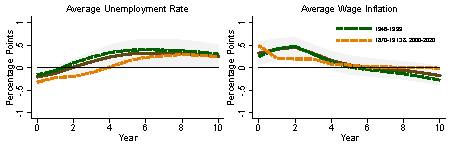
\includegraphics[width=\textwidth]{../Output/Figures/fig_full_SDLPIVBM10_2_asym_postwar.pdf}
		\end{subfigure}
		\annote{Phillips multiplier estimated using the trilemma IV as instrument according to Equation \eqref{EQ:MULT}. For the multiplier (upper-left), the shaded area corresponds to the 90\% confidence interval implied by the normal limiting distribution of the 2SLS estimator. The F-statistics (upper-right) are computed as discussed in \cite{Olea2013}. The impulse responses (bottom panels) for \textit{average} wage inflation and unemployment are obtained from the OLS regressions \eqref{EQ:IRF} and display 90\% confidence sets. Across all figures, one can distinguish the state by its color and shape, a short-dashed orange shape for the period with more credible anchored inflation (1870-1913 \& 2000-2019) and a long-dashed green shape for the post-war period (1946-1999).}
	
\end{figure}

Figure \ref{F2:Multiplier_M_GS} displays a bigger Phillips multiplier for the post-war period. Its difference becomes statistically significant from horizon $t=7$ onward with the weak instrument robust Anderson-Rubin p-values being 0.031, 0.019, 0.025, and 0.089 for horizons 7, 8, 9, and 10 respectively.\footnote{See Table \ref{T:SDPM_GS} in the Appendix for a more detailed description of this result.} This result is in line with the idea put forward by Figure \ref{F:RWIV} in which we see that the correlation between unemployment and wage inflation is weaker in the last 20 years and during the Gold Standard.

Figure \ref{F2:Dynamics_GS} indicates that the wage inflation response is the main driver of the weaker tradeoff in the credible inflation anchor periods. Although the average unemployment rate response is virtually identical in both the baseline and the state dependencies for longer horizons, the average wage inflation response is muted for longer horizons.

\begin{table}[ht]
\footnotesize
\centering
\def\sym#1{\ifmmode^{#1}\else\(^{#1}\)\fi}
\caption{Estimates of multipliers across sub-samples \label{T:SDPM_GS}}
\begin{tabular}{l*{1}{cccc}}
\hline\hline
 Horizon  & Linear & 1946-1999    & 1870-1913 \&   & AR            \\
          & Model  &              & 2000-2020      & p-value       \\
\hline
   4       & 0.499 & 0.383 & -0.154 & 0.310 \\
          & (0.629) & (0.581) & (0.191) & \\
 & & & &\\
   5       & 0.131 & 0.026 & -0.150 & 0.167 \\
          & (0.421) & (0.411) & (0.107) & \\
 & & & &\\
   6       & -0.010 & -0.109 & -0.211 & 0.091 \\
          & (0.343) & (0.336) & (0.076) & \\
 & & & &\\
   7       & -0.115 & -0.239 & -0.184 & 0.031 \\
          & (0.319) & (0.307) & (0.089) & \\
 & & & &\\
   8       & -0.217 & -0.374 & -0.169 & 0.019 \\
          & (0.317) & (0.308) & (0.104) & \\
 & & & &\\
   9       & -0.416 & -0.601 & -0.161 & 0.025 \\
          & (0.327) & (0.322) & (0.125) & \\
 & & & &\\
  10       & -0.757 & -0.945 & -0.292 & 0.089 \\
          & (0.388) & (0.407) & (0.116) & \\
 & & & &\\
\hline\hline
\end{tabular}

\annote{\footnotesize This table presents the multiplier estimates corresponding to the ones in Figure \ref{F2:Multiplier_M_GS}. The values in parentheses under the multipliers indicate the corresponding standard errors. The last column indicates the weak instrument robust Anderson-Rubin p-values for the difference in multipliers across states.}
\end{table}

\end{singlespace}


\end{comment}

\end{appendices}

\end{document}
